\documentclass[12pt,addpoints]{exam}
%-----------------------------------------------------------------------------
% PACKAGES AND OTHER DOCUMENT CONFIGURATIONS
%-----------------------------------------------------------------------------

\usepackage[margin=1in]{geometry}
\usepackage{amsmath, amsfonts}
\usepackage{enumerate}
\usepackage{graphicx}
\usepackage{titling}
\usepackage{url}
\usepackage{xfrac}
\usepackage{natbib}
\usepackage{amssymb}
\usepackage{amsthm}
\usepackage{paralist}
\usepackage{epstopdf}
\usepackage{tabularx}
\usepackage{longtable}
\usepackage{multirow}
\usepackage{multicol}
\usepackage[colorlinks=true,urlcolor=blue]{hyperref}
\usepackage{algorithm}
\usepackage{algorithmicx}
\usepackage[noend]{algpseudocode}
\usepackage{float}
\usepackage{enumerate}
\usepackage{array}
\usepackage{environ}
\usepackage{times}
\usepackage{textcomp}
\usepackage{caption}
\usepackage{parskip} % For NIPS style paragraphs.
\usepackage[compact]{titlesec} % Less whitespace around titles
\usepackage[inline]{enumitem} % For inline enumerate* and itemize*
\usepackage{datetime}
\usepackage{comment}
% \usepackage{minted}
\usepackage{lastpage}
\usepackage{color}
% \usepackage{xcolor}
\usepackage[dvipsnames]{xcolor}
\usepackage[final]{listings}
\usepackage{tikz}
\usetikzlibrary{shapes,decorations}
\usepackage{framed}
\usepackage{booktabs}
\usepackage{cprotect}
\usepackage{verbatimbox}
\usepackage{multicol}
\usepackage{hyperref}
\usepackage{subcaption}
\usepackage{mathtools} % For drcases
\usepackage{cancel}
\usepackage[many]{tcolorbox}
\tcbuselibrary{listings} % For listings within tcolorbox
\usepackage{soul}
\usepackage[bottom]{footmisc}
\usepackage{bm}
\usepackage{wasysym}
\usepackage{lipsum}

\usepackage{tikz}
\usetikzlibrary{arrows}
\usetikzlibrary{arrows.meta}
\usetikzlibrary{shapes.geometric}
\usetikzlibrary{positioning, arrows, automata, calc}
\usepackage{transparent}
\usepackage{tikz-cd}

%%%%%%%%%%%%%%%%%%%%%%%%%%%%%%%%%%%%%%%%%%%
% Formatting for \CorrectChoice of "exam" %
%%%%%%%%%%%%%%%%%%%%%%%%%%%%%%%%%%%%%%%%%%%

\CorrectChoiceEmphasis{}
\checkedchar{\blackcircle}

\newenvironment{checkboxessquare}{
    \begingroup
    \checkboxchar{$\Box$} \checkedchar{$\blacksquare$} % change checkbox style locally
    \begin{checkboxes}
    }{
    \end{checkboxes}
    \endgroup
    }

    
\newenvironment{oneparcheckboxessquare}{
    \begingroup
    \checkboxchar{$\Box$} \checkedchar{$\blacksquare$} % change checkbox style locally
    \begin{oneparcheckboxes}
    }{
    \end{oneparcheckboxes}
    \endgroup
    }

%%%%%%%%%%%%%%%%%%%%%%%%%%%%%%%%%%%%%%%%%%%
% Better numbering                        %
%%%%%%%%%%%%%%%%%%%%%%%%%%%%%%%%%%%%%%%%%%%

% \numberwithin{equation}{section} % Number equations within sections (i.e. 1.1, 1.2, 2.1, 2.2 instead of 1, 2, 3, 4)
% \numberwithin{figure}{section} % Number figures within sections (i.e. 1.1, 1.2, 2.1, 2.2 instead of 1, 2, 3, 4)
% \numberwithin{table}{section} % Number tables within sections (i.e. 1.1, 1.2, 2.1, 2.2 instead of 1, 2, 3, 4)

%%%%%%%%%%%%%%%%%%%%%%%%%%%%%%%%%%%%%%%%%%
% Custom commands                        %
%%%%%%%%%%%%%%%%%%%%%%%%%%%%%%%%%%%%%%%%%%
\newcommand{\blackcircle}{\tikz\draw[black,fill=black] (0,0) circle (1ex);}
\renewcommand{\circle}{\tikz\draw[black] (0,0) circle (1ex);}

\newcommand{\solo}{ \textcolor{orange}{[SOLO]} }
\newcommand{\open}{ \textcolor{blue}{[OPEN]} }

\input{../shared/mathabbreviations.tex}

%%%%%%%%%%%%%%%%%%%%%%%%%%%%%%%%%%%%%%%%%%%
% Code highlighting with listings         %
%%%%%%%%%%%%%%%%%%%%%%%%%%%%%%%%%%%%%%%%%%%

\definecolor{bluekeywords}{rgb}{0.13,0.13,1}
\definecolor{greencomments}{rgb}{0,0.5,0}
\definecolor{redstrings}{rgb}{0.9,0,0}
\definecolor{light-gray}{gray}{0.95}

\newcommand{\MYhref}[3][blue]{\href{#2}{\color{#1}{#3}}}%

\definecolor{dkgreen}{rgb}{0,0.6,0}
\definecolor{gray}{rgb}{0.5,0.5,0.5}
\definecolor{mauve}{rgb}{0.58,0,0.82}

\lstdefinelanguage{Shell}{
  keywords={tar, cd, make},
  %keywordstyle=\color{bluekeywords}\bfseries,
  alsoletter={+},
  ndkeywords={python3, python, py, javac, java, gcc, c, g++, cpp, .txt, octave, m, .tar},
  %ndkeywordstyle=\color{bluekeywords}\bfseries,
  identifierstyle=\color{black},
  sensitive=false,
  comment=[l]{//},
  morecomment=[s]{/*}{*/},
  commentstyle=\color{purple}\ttfamily,
  %stringstyle=\color{red}\ttfamily,
  morestring=[b]',
  morestring=[b]",
  backgroundcolor = \color{light-gray}
}

\lstset{columns=fixed, basicstyle=\ttfamily,
    backgroundcolor=\color{light-gray},xleftmargin=0.5cm,frame=tlbr,framesep=4pt,framerule=0pt}

\newcommand{\emptysquare}{{\LARGE $\square$}\ \ }
\newcommand{\filledsquare}{{\LARGE $\boxtimes$}\ \ }
\def \ifempty#1{\def\temp{#1} \ifx\temp\empty }


% \newcommand{\squaresolutionspace}[2][\emptysquare]{\newline #1}{#2}
\def \squaresolutionspace#1{ \ifempty{#1} \emptysquare \else #1\hspace{0.75pt}\fi}
\newcommand{\squaresoln}[0]{ \begin{soln}\filledsquare \end{soln}}


\newcommand{\emptycircle}{{\LARGE $\fullmoon$}\ \ }
\newcommand{\filledcircle}{{\LARGE $\newmoon$}\ \ }
\def \circlesolutionspace#1{ \ifempty{#1} \emptycircle \else #1\hspace{0.75pt}\fi}
\newcommand{\circlesoln}[0]{ \begin{soln}\filledcircle \end{soln}}
%%%%%%%%%%%%%%%%%%%%%%%%%%%%%%%%%%%%%%%%%%%
% Custom box for highlights               %
%%%%%%%%%%%%%%%%%%%%%%%%%%%%%%%%%%%%%%%%%%%

% Define box and box title style
\tikzstyle{mybox} = [fill=blue!10, very thick,
    rectangle, rounded corners, inner sep=1em, inner ysep=1em]

% \newcommand{\notebox}[1]{
% \begin{tikzpicture}
% \node [mybox] (box){%
%     \begin{minipage}{\textwidth}
%     #1
%     \end{minipage}
% };
% \end{tikzpicture}%
% }

\NewEnviron{notebox}{

\begin{tikzpicture}
\node [mybox] (box){
    \begin{minipage}{0.95\textwidth}
        \BODY
    \end{minipage}
};
\end{tikzpicture}
}

%%%%%%%%%%%%%%%%%%%%%%%%%%%%%%%%%%%%%%%%%%%
% Commands showing / hiding solutions     %
%%%%%%%%%%%%%%%%%%%%%%%%%%%%%%%%%%%%%%%%%%%
\newcommand{\solutionspace}[4]{\fbox{\begin{minipage}[t][#1][t]{#2} \textbf{#3} \solution{}{#4} \end{minipage}}}

% To HIDE SOLUTIONS, set this value to 0:
%\providecommand{\issoln}{0}
%\providecommand{\issoln}{1}

\ifthenelse{\equal{\issoln}{1}}{

% SOLUTION environment
\newenvironment{soln}{\leavevmode\color{red}\ignorespaces }{}

% QUESTION AUTHORS environment
\newenvironment{qauthor}{\leavevmode\color{blue}\ignorespaces }{}

% Question tester comment environment
\newenvironment{qtester}{\leavevmode\color{green}\ignorespaces}{}

% Question learning objective comment environment
\newenvironment{qlearningobjective}{\leavevmode\color{green}\ignorespaces}{}

}{ % ELSE

  \NewEnviron{soln}{}
  \NewEnviron{qauthor}{}
  \NewEnviron{qtester}{}
  \NewEnviron{qlearningobjective}{}

}

%% To HIDE TAGS set this value to 0:
\def\showtags{0}
%%%%%%%%%%%%%%%%
\ifcsname showtags\endcsname \else \def\showtags{1} \fi
% Default to an empty tags environ.
\NewEnviron{tags}{}{}
\if\showtags 1
% Otherwise, include solutions as below.
\RenewEnviron{tags}{
    \fbox{
    \leavevmode\color{blue}\ignorespaces
    \textbf{TAGS:} \texttt{\url{\BODY}}
    }
    \vspace{-.5em}
}{}
\fi

\newtcolorbox[]{answer_box}[1][]
{
    % breakable,
    fit,
    enhanced,
    % nobeforeafter,
    colback=white,
    title=Your Answer,
    sidebyside align=top,
    box align=top,
    #1
}

% This must be specified with option brackets \begin{answerboxcode}[] \end{answerboxcode}
% For some reason, this would break if we used the name answer_box_code
\newtcblisting{answerboxcode}[1][]
{
    listing only,
    listing options={
        language=Python,
        showstringspaces=false,     % Don't show spaces in strings
        tabsize=4,                  % Set tab size to 4 spaces
        breaklines=true,            % Break long lines
        numbers=left,               % Line numbers on the left
    },
    height=6cm,
    width=15cm,
    fit,
    enhanced,
    colback=white,
    title=Your Answer,
    sidebyside align=top,
    box align=top,
    #1
}

%\pagestyle{fancyplain}
\lhead{\hwName{}
\begin{soln}Solutions\end{soln}
}
\rhead{\courseNum}
\cfoot{\thepage{} of \numpages{}}

\title{\textsc{\hwNum}
\begin{soln}Solutions\end{soln}
\\
\textsc{\hwTopic}
\thanks{Compiled on \today{} at \currenttime{}}\\
\vspace{1em}
} % Title


\author{\textsc{\large \courseNum{} \courseName{}}\\
\courseUrl
\vspace{1em}\\
\ifdefempty{\outDate}{}{  OUT: \outDate \\ }
\ifdefempty{\dueDate}{}{  DUE: \dueDate \\ }
\ifdefempty{\taNames}{}{  TAs: \taNames{} }
}

\date{}

%%%%%%%%%%%%%%%%%%%%%%%%%%%%%%%%%%%%%%%%%%%%%%%%%
% Useful commands for typesetting the questions %
%%%%%%%%%%%%%%%%%%%%%%%%%%%%%%%%%%%%%%%%%%%%%%%%%

% This command will allow long \lstinline{} text to wrap automatically.
\sloppy

%%%%%%%%%%%%%%%%%%%%%%%%%%
% Document configuration %
%%%%%%%%%%%%%%%%%%%%%%%%%%

% Don't display a date in the title and remove the white space
\predate{}
\postdate{}
\date{}

% Don't display an author and remove the white space
% \preauthor{}
% \postauthor{}

% Question type commands
\newcommand{\sall}{\textbf{Select all that apply: }}
\newcommand{\sone}{\textbf{Select one: }}
\newcommand{\tf}{\textbf{True or False: }}




% Changes to examdoc
\qformat{\textbf{{\Large \thequestion \; \; \thequestiontitle \ (\totalpoints \ points)}} \hfill}
\renewcommand{\thequestion}{\arabic{question}}
\renewcommand{\questionlabel}{\thequestion.}

\renewcommand{\thepartno}{\thequestion.\arabic{partno}}
%\renewcommand{\partlabel}{\thequestion.\thepartno.}
\renewcommand{\partlabel}{\thepartno.}

% not working: \renewcommand{\subpartlabel}{(\thequestion.\thepartno.\thesubpart)}
% Commented after adding \question.\thepartno.
%\renewcommand{\partshook}{\setlength{\leftmargin}{0pt}}

\renewcommand{\thesubpart}{\thepartno.\alph{subpart}}
\renewcommand{\subpartlabel}{\thesubpart.}

\renewcommand{\thesubsubpart}{\thesubpart.\roman{subsubpart}}
\renewcommand{\subsubpartlabel}{\thesubsubpart.}

% copied from stack overflow, as all good things are
\newcommand\invisiblesection[1]{%
  \refstepcounter{section}%
  \addcontentsline{toc}{section}{\protect\numberline{\thesection}#1}%
  \sectionmark{#1}}

% quite possibly the worst workaround i have made for this class
\newcommand{\sectionquestion}[1]{
\titledquestion{#1}
\invisiblesection{#1}
~\vspace{-1em}
}

%%%%%%%%%%%%%%%%%%%%%%%%%%%%%%%%%%%%%%%%%%%
% New Environment for Pseudocode          %
%%%%%%%%%%%%%%%%%%%%%%%%%%%%%%%%%%%%%%%%%%%

% Python style for highlighting
\DeclareFixedFont{\ttb}{T1}{txtt}{bx}{n}{12} % for bold
\DeclareFixedFont{\ttm}{T1}{txtt}{m}{n}{12}  % for normal

\definecolor{deepblue}{rgb}{0,0,0.5}
\definecolor{deepred}{rgb}{0.6,0,0}
\definecolor{deepgreen}{rgb}{0,0.5,0}

\newcommand\pythonstyle{\lstset{
language=Python,
basicstyle=\ttm,
morekeywords={self},              % Add keywords here
keywordstyle=\ttb\color{deepblue},
emph={MyClass,__init__},          % Custom highlighting
emphstyle=\ttb\color{deepred},    % Custom highlighting style
stringstyle=\color{deepgreen},
frame=tb,                         % Any extra options here
showstringspaces=false
}}


% Python environment
\lstnewenvironment{your_code_solution}[1][]
{
\pythonstyle
\lstset{#1}
}
{}


\begin{document}

\begin{soln}{\huge \bf Solutions}\end{soln}

\newcommand{\toreplace}[1]{#1}
\renewcommand{\toreplace}[1]{\underline{\hspace{10em}}}
\renewcommand{\toreplace}[1]{\hphantom{\hspace{5em}}}


\pagestyle{head}
\firstpageheader{}{}{}
\runningheader{\class}{\examnum\ - Page \thepage\ of \numpages}{ID: zhuyunj - 330}
\runningheadrule

% Default to an empty tags environ.
\NewEnviron{tags}{}{}

\noindent
\begin{tabular*}{\textwidth}{l @{\extracolsep{3cm}} r @{\extracolsep{6pt}} l}
\textbf{\class} & \textbf{Name:} & {Zhuyun Jin}\\
\textbf{\term} &  \textbf{Andrew ID:} & {zhuyunj} \\
\textbf{\examnum} & \textbf{Room:} & {DH A302}\\
\textbf{\examdate} & \textbf{Seat:} & {F03} \\
\textbf{Time Limit: \timelimit} & \textbf{Exam Number:} & {330}
\end{tabular*}\\
\rule[2ex]{\textwidth}{2pt}

\textbf{Instructions:}
\begin{itemize}
    \item Verify your name and Andrew ID above. 
    \item This exam contains \numpages\ pages (including this cover page).\\
    The total number of points is \numpoints. 
    %The total number of questions is \numquestions.
    %\item You are allowed to use one page of notes
    \item Clearly mark your answers in the allocated space If you have made a mistake, cross out the invalid parts of your solution, and circle the ones which should be graded.
    \item Look over the exam first to make sure that none of the \numpages\ pages are missing. 
    \item No electronic devices may be used during the exam.
    \item Please write all answers \emph{darkly} in pencil or in pen.
    \item You have \timelimit{} to complete the exam. Good luck!
\end{itemize}

\begin{center}
    \pointtable[v][questions]
\end{center}

\noindent
\rule[2ex]{\textwidth}{2pt}
\newpage

\section*{Instructions for Specific Problem Types}

For ``Select One" questions, please fill in the appropriate bubble completely:

\begin{quote}
\textbf{Select One:} Who taught this course?
    \begin{list}{}
     \item\CIRCLE{} Matt Gormley
     \item\Circle{} Marie Curie
     \item\Circle{} Noam Chomsky
    \end{list}
\end{quote}

If you need to change your answer, you may cross out the previous answer and bubble in the new answer:

\begin{quote}
\textbf{Select One:} Who taught this course?
    \begin{list}{}
     \item\CIRCLE{} Henry Chai
     \item\Circle{} Marie Curie \\[0.25cm]
     \xcancel{\CIRCLE}{} Noam Chomsky
    \end{list}
\end{quote}

For ``Select all that apply" questions, please fill in all appropriate squares completely:

\begin{quote}
\textbf{Select all that apply:} Which are instructors for this course?
    \begin{list}{}
    \item $\blacksquare$ Matt Gormley  
    \item $\blacksquare$ Henry Chai
    \item $\blacksquare$  Hoda Heidari
    \item $\square$ I don't know
    \end{list}
\end{quote}

Again, if you need to change your answer, you may cross out the previous answer(s) and bubble in the new answer(s):

\begin{quote}
\textbf{Select all that apply:} Which are the instructors for this course?
    \begin{list}{}
    \item $\blacksquare$ Matt Gormley 
    \item $\blacksquare$ Henry Chai
    \item $\blacksquare$ Hoda Heidari \\[0.25cm]
    \xcancel{$\blacksquare$} I don't know
    \end{list}
\end{quote}

For questions where you must fill in a blank, please make sure your final answer is fully included in the given space. You may cross out answers or parts of answers, but the final answer must still be within the given space.

\begin{quote}
\textbf{Fill in the blank:} What is the course number?

\begin{tcolorbox}[fit,height=1cm, width=4cm, blank, borderline={1pt}{-2pt},nobeforeafter]
    \begin{center}\huge10-601\end{center}
    \end{tcolorbox}\hspace{2cm}
    \begin{tcolorbox}[fit,height=1cm, width=4cm, blank, borderline={1pt}{-2pt},nobeforeafter]
    \begin{center}\huge10-\xcancel{6}301\end{center}
    \end{tcolorbox}
\end{quote}

\clearpage
\begin{questions}
%\sectionquestion{Question Template - FOR INSTRUCTOR USE}

\textbf{Format your question types as shown below.}

\begin{parts}

\part[1] \textbf{True or False:} Input question here.
    \begin{checkboxes}
     \choice True 
     \choice False
    \end{checkboxes}
    \begin{soln}
    Input solution here.
    \end{soln}
    \begin{qauthor}
    Input (1) author name, (2) learning objective addressed, and (3) source if  adapting/reusing a question.
    \end{qauthor}

\part[1] \textbf{Select one:} Input question here
    \begin{checkboxes}
     \choice Stephen Hawking 
     \choice Albert Einstein
     \choice Isaac Newton
     \choice I don't know
    \end{checkboxes}
    \begin{soln}
    Input solution here.
    \end{soln}
    \begin{qauthor}
    Input (1) author name, (2) learning objective addressed, and (3) source if  adapting/reusing a question.
    \end{qauthor}
    
\part[1] \textbf{Select all that apply:} Input question here.
    \begin{checkboxessquare}
     \choice Stephen Hawking 
     \choice Albert Einstein
     \choice Isaac Newton
     \choice None of the above
    \end{checkboxessquare}
    \begin{soln}
    Input solution here.
    \end{soln}
    \begin{qauthor}
    Input (1) author name, (2) learning objective addressed, and (3) source if  adapting/reusing a question.
    \end{qauthor}
    
\part[1] \textbf{Fill in the blank:} \textit{Input your \underline{\hspace{8em}} here.}
    \begin{checkboxes}
     \choice money 
     \choice dignity
     \choice question
     \choice I don't know
    \end{checkboxes}
    \begin{soln}
    Input solution here.
    \end{soln}
    \begin{qauthor}
    Input (1) author name, (2) learning objective addressed, and (3) source if  adapting/reusing a question.
    \end{qauthor}
        
\part[1] \textbf{Numerical answer:} Input your question here.
    \begin{answer_box}[title=,height=1cm, width=2cm]
    \end{answer_box}
    \begin{soln}
    Input solution here.
    \end{soln}
    \begin{qauthor}
    Input (1) author name, (2) learning objective addressed, and (3) source if  adapting/reusing a question.
    \end{qauthor}

    
\part[1] \textbf{Ordering:}  Input your question here. 
\textit{Select the correct ordering of the items below by numbering them from 1 to 3.}
    \begin{itemize}
        \item Something 
            \begin{answer_box}[title=,height=1cm, width=2cm,nobeforeafter,box align=center]
            \end{answer_box}
        \item Another thing 
            \begin{answer_box}[title=,height=1cm, width=2cm,nobeforeafter,box align=center]
            \end{answer_box}
        \item Still another
            \begin{answer_box}[title=,height=1cm, width=2cm,nobeforeafter,box align=center]
            \end{answer_box}
    \end{itemize}
    \begin{soln}
    Input solution here.
    \end{soln}
    \begin{qauthor}
    Input (1) author name, (2) learning objective addressed, and (3) source if  adapting/reusing a question.
    \end{qauthor}

\part[1] \textbf{Short answer:} Input your question here.
    \fillwithlines{8em}
    \begin{soln}
    Input solution here.
    \end{soln}
    \begin{qauthor}
    Input (1) author name, (2) learning objective addressed, and (3) source if  adapting/reusing a question.
    \end{qauthor}
    
\part[1] \textbf{Derivation:} Input your question here.
    \begin{answer_box}[title=,height=5cm, width=15cm]
    \end{answer_box}
    \begin{soln}
    Input solution here.
    \end{soln}
    \begin{qauthor}
    Input (1) author name, (2) learning objective addressed, and (3) source if  adapting/reusing a question.
    \end{qauthor}

\part[1] \textbf{Proof:} Input your question here.
    \begin{answer_box}[title=,height=5cm, width=15cm]
    \end{answer_box}
    \begin{soln}
    Input solution here.
    \end{soln}
    \begin{qauthor}
    Input (1) author name, (2) learning objective addressed, and (3) source if  adapting/reusing a question.
    \end{qauthor}

\part \textit{For questions like this one that require some preamable, you should rely on the parts environment.} Consider the function $f(x)=3x^3+2x^2+x+1$. Do NOT include points on the \textit{question}, only on the \textit{part}.
    \begin{subparts}
    \subpart[10] \textit{Here you drop in one of the question templates above, replacing the question command with the part command.} Calculate $f'(x)$.
    \addpoints
    \subpart[10] \textit{Here you drop in one of the question templates above, replacing the question command with the part command.} Calculate $f''(x)$.
    \end{subparts}

\end{parts}

%\clearpage
%\input{qs-TA-s24.tex}
%\clearpage
% \sectionquestion{Regression and Optimization}

\begin{parts}

\part Suppose you have a regression dataset with one input feature, $x$, and one output value $y$. You wish to evaluate various regression techniques.

\begin{subparts}
    \subpart[2] \textbf{Drawing:} Draw the function that a linear regression model would learn on the dataset below.

    \begin{center}
    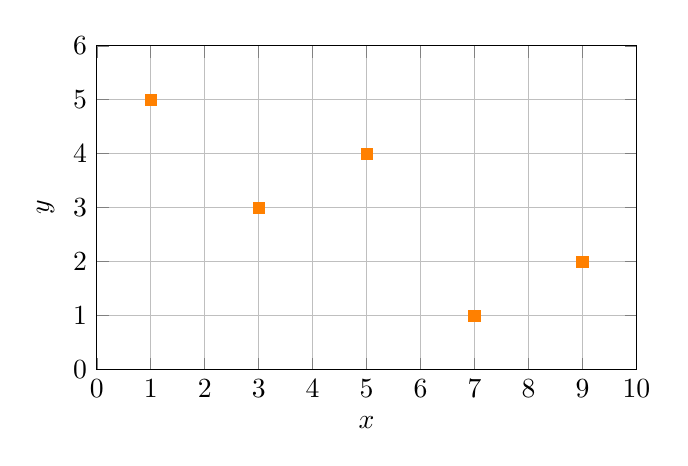
\begin{tikzpicture}
    \begin{axis}[
        scale=1.0, axis equal image,
        xmin=0, xmax=10, xtick={0,...,10},
        ymin=0, ymax=6, ytick={0,...,6},
        samples=50, grid=major, xlabel=$x$, ylabel=$y$]
        \addplot [
            scatter,
            only marks,
            point meta=explicit symbolic,
            scatter/classes={
                a={mark=square*,orange},
                b={mark=triangle*,red}
            },
            nodes near coords*={},
            visualization depends on={\thisrow{myvalue} \as \myvalue},
        ] table [meta=label] {
            x y label myvalue
            1 5 a 1
            3 3 a 1
            5 4 a 1
            7 1 a 1
            9 2 a 1
        };
    \end{axis}
    \end{tikzpicture}
    \end{center}
    \begin{soln} Any straight line that roughly passes through the points should get full credit. \end{soln}
    \begin{qauthor} Matt (Solution by Henry) \end{qauthor}

    \subpart[2] \textbf{Drawing:} Draw the function that a $k$-nearest neighbor regression model with $k=1$ would learn on the dataset below.

    \begin{center}
    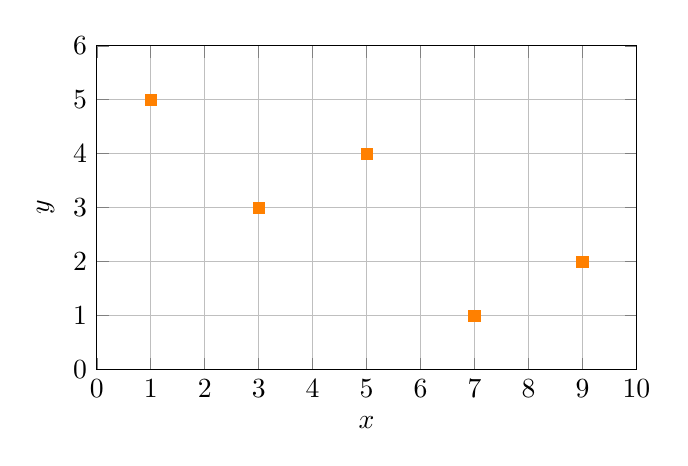
\begin{tikzpicture}
    \begin{axis}[
        scale=1.0, axis equal image,
        xmin=0, xmax=10, xtick={0,...,10},
        ymin=0, ymax=6, ytick={0,...,6},
        samples=50, grid=major, xlabel=$x$, ylabel=$y$]
        \addplot [
            scatter,
            only marks,
            point meta=explicit symbolic,
            scatter/classes={
                a={mark=square*,orange},
                b={mark=triangle*,red}
            },
            nodes near coords*={},
            visualization depends on={\thisrow{myvalue} \as \myvalue},
        ] table [meta=label] {
            x y label myvalue
            1 5 a 1
            3 3 a 1
            5 4 a 1
            7 1 a 1
            9 2 a 1
        };
    \end{axis}
    \end{tikzpicture}
    \end{center}
    \begin{soln} Piecewise linear with all components parallel to the x-axis, passing through the points, i.e., line segment from $x\in [0,2]$ at $y=5$, then $x\in [2,4]$ at $y=3$ etc... \end{soln}
    \begin{qauthor} Matt (Solution by Henry) \end{qauthor}
    
    \subpart[2] \textbf{Drawing:} Draw the function that a decision tree regression model with features of the form $x < c$ would learn on the dataset below.

    \begin{center}
    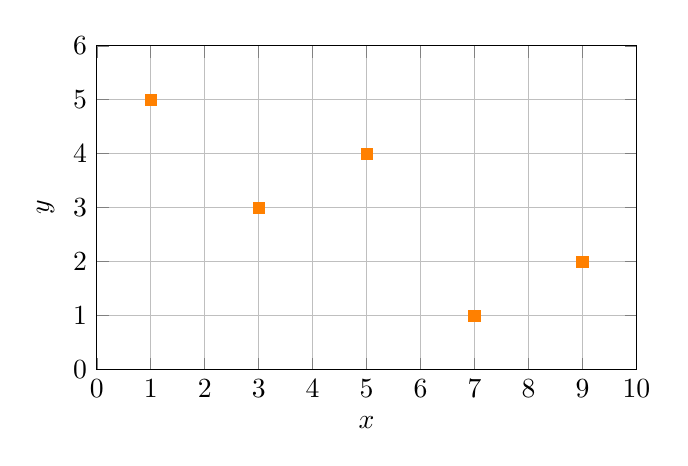
\begin{tikzpicture}
    \begin{axis}[
        scale=1.0, axis equal image,
        xmin=0, xmax=10, xtick={0,...,10},
        ymin=0, ymax=6, ytick={0,...,6},
        samples=50, grid=major, xlabel=$x$, ylabel=$y$]
        \addplot [
            scatter,
            only marks,
            point meta=explicit symbolic,
            scatter/classes={
                a={mark=square*,orange},
                b={mark=triangle*,red}
            },
            nodes near coords*={},
            visualization depends on={\thisrow{myvalue} \as \myvalue},
        ] table [meta=label] {
            x y label myvalue
            1 5 a 1
            3 3 a 1
            5 4 a 1
            7 1 a 1
            9 2 a 1
        };
    \end{axis}
    \end{tikzpicture}
    \end{center}
    \begin{soln} Very similar to part (b) except the line segments to do not need to end exactly at the midpoints between the orange squares; should still be piecewise linear with components parallel to the x-axis. \end{soln}
    \begin{qauthor} Matt (Solution by Henry) \end{qauthor}
\end{subparts}
    
\part We wish to learn a linear regression model on data $\Dc = \{ (\xv^{(i)}, y^{(i)}) \}_{i=1}^N$ For this question, define the pointwise exponential squared error as
\[
    J^{(i)}\Big(\thetav\Big)=\textrm{exp}\bigg(\frac{1}{2}\Big(y^{(i)} - \thetav^T\xv^{(i)}\Big)^2\bigg)
\]
Suppose we are interested in minimizing the \emph{geometric} mean of the exponential squared errors over our training data. Recall that the geometric mean of a set of values \\ $\{x^{(1)}, \ldots, x^{(n)}\}$ is the $n^{\textrm{th}}$ root of their product. Thus, our objective in this setting is
\[
    J\Big(\thetav\Big)=\bigg(\prod_{i=1}^N J^{(i)}(\thetav)\bigg)^{\frac{1}{N}}
\]

\begin{subparts}
    \subpart[2] \textbf{Math:} What is the partial derivative of $J^{(i)}\Big(\thetav\Big)$ with respect to the $k^{\textrm{th}}$ parameter, $\theta_k$?
    \begin{tcolorbox}[fit,height=3cm, width=15cm, blank, borderline={1pt}{-2pt}]
        %solution
    \end{tcolorbox}
    \begin{soln}
        \begin{align}
            \frac{\partial J^{(i)}}{\partial \theta_j} &= \frac{\partial}{\partial \theta_j}\Bigg(\textrm{exp}\bigg(\frac{1}{2}\Big(y^{(i)} - \vec{\theta}^T\vec{x}^{(i)}\Big)^2\bigg)\Bigg) \nonumber \\ 
            &= \textrm{exp}\bigg(\frac{1}{2}\Big(y^{(i)} - \vec{\theta}^T\vec{x}^{(i)}\Big)^2\bigg)\frac{\partial}{\partial \theta_j}\frac{1}{2}\Big(y^{(i)} - \vec{\theta}^T\vec{x}^{(i)}\Big)^2 \nonumber \\
            &= \textrm{exp}\bigg(\frac{1}{2}\Big(y^{(i)} - \vec{\theta}^T\vec{x}^{(i)}\Big)^2\bigg)\Big(y^{(i)} - \vec{\theta}^T\vec{x}^{(i)}\Big)\Big(-x^{(i)}_j\Big) \nonumber
        \end{align}
    \end{soln}
    \begin{qauthor}
       Henry
    \end{qauthor}
    
    \subpart[2] \textbf{Math:} What is the gradient of $J^{(i)}\Big(\thetav\Big)$ with respect to the vector $\thetav$?
    \begin{tcolorbox}[fit,height=3cm, width=15cm, blank, borderline={1pt}{-2pt}]
        %solution
    \end{tcolorbox}
    \begin{soln}
        \begin{align}
            \frac{\partial J^{(i)}}{\partial \vec{\theta}} &= \frac{\partial}{\partial \vec{\theta}}\Bigg(\textrm{exp}\bigg(\frac{1}{2}\Big(y^{(i)} - \vec{\theta}^T\vec{x}^{(i)}\Big)^2\bigg)\Bigg) \nonumber \\ 
            &= \textrm{exp}\bigg(\frac{1}{2}\Big(y^{(i)} - \vec{\theta}^T\vec{x}^{(i)}\Big)^2\bigg)\frac{\partial}{\partial \vec{\theta}}\frac{1}{2}\Big(y^{(i)} - \vec{\theta}^T\vec{x}^{(i)}\Big)^2 \nonumber \\
            &= \textrm{exp}\bigg(\frac{1}{2}\Big(y^{(i)} - \vec{\theta}^T\vec{x}^{(i)}\Big)^2\bigg)\Big(y^{(i)} - \vec{\theta}^T\vec{x}^{(i)}\Big)\Big(-\vec{x}^{(i)}\Big) \nonumber
        \end{align}
    \end{soln}
    \begin{qauthor}
       Henry
    \end{qauthor}
    
    % \part[1] \textbf{Select one:} Using the design matrix, $X$, and the vector of outputs, $\vec{y}$, which of the following is the gradient of $J\Big(\vec{\theta}\Big)$ with respect to the vector $\vec{\theta}$? 
    % \begin{checkboxes}
    %    \choice $\textrm{exp}\bigg(\frac{1}{2N}\Big(X\vec{\theta} - \vec{y}\Big)^T\Big(X\vec{\theta} - \vec{y}\Big)\bigg)\frac{1}{N}\big(X^TX\vec{\theta}-X^T\vec{y}\big)$ 
    %    \choice $\textrm{exp}\bigg(\frac{1}{2N}\Big(X\vec{\theta} - \vec{y}\Big)^T\Big(X\vec{\theta} - \vec{y}\Big)\bigg)\frac{1}{2N}\Big(X\vec{\theta} - \vec{y}\Big)^T\Big(X\vec{\theta} - \vec{y}\Big)$
    %    \choice $\textrm{exp}\bigg(\frac{1}{N}\big(X^TX\vec{\theta}-X^T\vec{y}\big)\bigg)\frac{1}{2N}\Big(X\vec{\theta} - \vec{y}\Big)^T\Big(X\vec{\theta} - \vec{y}\Big)$
    %    \choice $\textrm{exp}\bigg(\frac{1}{N}\big(X^TX\vec{\theta}-X^T\vec{y}\big)\bigg)\frac{1}{N}\big(X^TX\vec{\theta}-X^T\vec{y}\big)$ 
    % \end{checkboxes}
    % \begin{soln}
    %    Making use of some exponential identities, we can rewrite $J\Big(\vec{\theta}\Big)$ as 
    %    \begin{align}
    %J^{(i)}(\vec{\theta})\bigg)^{\frac{1}{N}} \nonumber \\
    %        &= \Bigg(\prod_{i=1}^N \textrm{exp}\bigg(\frac{1}{2}\Big(y^{(i)} - \vec{\theta}^T\vec{x}^{(i)}\Big)^2\bigg)\Bigg)^{\frac{1}{N}} \nonumber \\
    %        &= \Bigg(\textrm{exp}\bigg(\sum_{i=1}^N \frac{1}{2}\Big(y^{(i)} - \vec{\theta}^T\vec{x}^{(i)}\Big)^2\bigg)\Bigg)^{\frac{1}{N}} \nonumber \\
    %        &= \textrm{exp}\bigg(\frac{1}{N}\sum_{i=1}^N \frac{1}{2}\Big(y^{(i)} - \vec{\theta}^T\vec{x}^{(i)}\Big)^2\bigg) \nonumber
    %    \end{align}
    %    which we can recognize as just the mean squared error exponentiated. Thus, the gradient of $J\Big(\vec{\theta}\Big)$ with respect to the vector $\vec{\theta}$ is
    %    \begin{align}
    %        \frac{\partial J}{\partial \vec{\theta}} &= \frac{\partial}{\partial \vec{\theta}}\textrm{exp}\bigg(\frac{1}{N}\sum_{i=1}^N \frac{1}{2}\Big(y^{(i)} - \vec{\theta}^T\vec{x}^{(i)}\Big)^2\bigg) \nonumber \\ 
    %        &= \textrm{exp}\bigg(\frac{1}{N}\sum_{i=1}^N \frac{1}{2}\Big(y^{(i)} - \vec{\theta}^T\vec{x}^{(i)}\Big)^2\bigg)\frac{1}{N} \frac{\partial}{\partial \vec{\theta}}\sum_{i=1}^N \frac{1}{2}\Big(y^{(i)} - \vec{\theta}^T\vec{x}^{(i)}\Big)^2 \nonumber \\
    %        &= \textrm{exp}\bigg(\frac{1}{2N}\Big(X\vec{\theta} - \vec{y}\Big)^T\Big(X\vec{\theta} - \vec{y}\Big)\bigg)\frac{1}{N}\big(X^TX\vec{\theta}-X^T\vec{y}\big) \nonumber
    %    \end{align}
    % \end{soln}
    % \begin{qauthor}
    %    Henry
    % \end{qauthor}
    
    Using the design matrix, $X$, and the vector of outputs, $\yv$, we can express the gradient of $J\Big(\thetav\Big)$ with respect to the vector $\thetav$ as
    \[
        \nabla_{\thetav} J\Big(\thetav\Big) = \textrm{exp}\bigg(\frac{1}{2N}\Big(X\thetav - \yv\Big)^T\Big(X\thetav - \yv\Big)\bigg)\frac{1}{N}\big(X^TX\thetav-X^T\yv\big)
    \]
    
    % \part[2] What is the closed-form solution for the optimal parameter vector $\vec{\theta}^*=\textrm{argmin }J\Big(\vec{\theta}\Big)$?
    % \begin{tcolorbox}[fit,height=3cm, width=15cm, blank, borderline={1pt}{-2pt}]
        % solution
    % \end{tcolorbox}
    
    \subpart[1] \textbf{True or False:} The optimal parameter vector in this setting is $\hat{\thetav} = \big(X^TX)^{-1}X^T\yv$, the same as the optimal parameter vector for minimizing the mean squared error.
    \begin{checkboxes}
        \choice True 
        \choice False
    \end{checkboxes}
    \begin{soln}
        True; because $\exp(x) > 0$ $\forall$ $x$, when we set the gradient above equal to zero, we can divide both sides by the exponential term and recover the OLS solution: 
        \[
            \thetav^*=\big(X^TX)^{-1}X^T\yv
        \]
    \end{soln}
    \begin{qauthor}
       Henry
    \end{qauthor}
\end{subparts}

\clearpage

\part[1] \textbf{Select one:} How many parameters does a linear regression model on 1-dimensional inputs have?
\begin{checkboxes}
    \choice $0$
    \choice $1$
    \choice $2$ 
    \choice $3$ 
\end{checkboxes}
\begin{soln}
    C
\end{soln}
\begin{qauthor}
   Henry
\end{qauthor}

\part You decide to optimize the function $f(x)=x^2$ with respect to $x$ using gradient descent. You initialize $x^{(0)}$ to $1$ and use a step size of $\eta = 2$. 

\begin{subparts}
\subpart[2] \textbf{Math:} Fill in the table below with the results you get from running gradient descent in this setting for two iterations (most of the $0^{\textrm{th}}$ iteration has been filled in on your behalf; you should fill in the missing element in this line along with all the other missing elements).

\begingroup
\renewcommand{\arraystretch}{2}
\begin{center}
\begin{tabular}{c|c|c|c}
    $t$ & $x^{(t)}$ & $f(x^{(t)})$ & $\nabla_x f(x^{(t)})$ \\ \hline
    0 & 1 & 1 & \underline{\qquad\qquad} \\ 
    1 & \underline{\qquad\qquad} & \underline{\qquad\qquad} & \underline{\qquad\qquad} \\ 
    2 & \underline{\qquad\qquad} & \underline{\qquad\qquad} & \underline{\qquad\qquad}
\end{tabular}
\end{center}
\endgroup

\begin{soln}
    \begingroup
    \renewcommand{\arraystretch}{2}
    \begin{center}
    \begin{tabular}{c|c|c|c}
        $t$ & $x^{(t)}$ & $f(x^{(t)})$ & $\nabla_x f(x^{(t)})$ \\ \hline
        0 & 1 & 1 & 2 \\ 
        1 & -3 & 9 & -6 \\ 
        2 & 9 & 81 & 18
    \end{tabular}
    \end{center}
    \endgroup
\end{soln}
\begin{qauthor}
    Henry
\end{qauthor}

\subpart[2] \textbf{Select all that apply:} Based on your findings from the previous question, which of the following changes could you make to achieve better results?
{%
\checkboxchar{$\Box$} \checkedchar{$\blacksquare$} % change checkbox style locally
\begin{checkboxes}
    \choice Run gradient descent for more iterations
    \choice Move the initial value $x^{(0)}$ closer towards (but not all the way to) the origin
    \choice Decrease the step size
    \choice Move in the direction of the gradient instead of in the opposite direction of the gradient
    \choice None of the above
\end{checkboxes}
}
\begin{soln}
   C; This step size is too large so decreasing it to anything $<1$ would improve the results. 
\end{soln}
\begin{qauthor}
    Henry (lightly edited from an M22 question)
\end{qauthor}
\end{subparts}

\end{parts}
% \clearpage
\sectionquestion{Optimization, Regularization, and Modeling}

\begin{parts}
\part Suppose you are given a dataset of $N$ data points $(x^{(i)},y^{(i)})_{i=1}^N$ where $x^{(i)},y^{(i)} \in \mathbb{R}$ and you fit a linear regression model to this dataset with no bias term and L2 regularization, i.e., you minimize the following objective function for:
\begin{equation*}
    J(\theta) = \frac{1}{N} \sum_{i=1}^n \left(\frac{1}{2} \left(y^{(i)}-\theta x^{(i)}\right)^2 \right) + \frac{\lambda}{2} \theta^2
\end{equation*}

\begin{subparts}
    \subpart[2] \textbf{Math:} What is $\frac{\partial J(\theta)}{\partial \theta}$? \textbf{You do not need to show your work for this problem.}
    \begin{tcolorbox}[fit,height=4cm, width=15cm, blank, borderline={1pt}{-2pt}]
        \begin{soln}
            \begin{equation*}
                \frac{\partial J(\theta)}{\partial \theta} = \frac{1}{N} \left(\sum_{i=1}^N \left(\theta {x^{(i)}}^2- x^{(i)} y^{(i)}\right)\right) + \lambda \theta
            \end{equation*}
        \end{soln}
    \end{tcolorbox}
        
    \subpart[2] \textbf{Math:} Find the closed form solution for $\hat{\theta}$, the optimal value of $\theta$. \textbf{Again, you do not need to show your work for this problem.}
    \begin{tcolorbox}[fit,height=4cm, width=15cm, blank, borderline={1pt}{-2pt}]
        \begin{soln}
            \begin{equation*}
                \hat{\theta} = \frac{\sum_{i=1}^N x^{(i)}y^{(i)}}{\sum_{i=1}^N {x^{(i)}}^2 + N\lambda}
            \end{equation*}
        \end{soln}
    \end{tcolorbox}
    
    \subpart[2] \textbf{Drawing:} Suppose you train several linear regression models on the same dataset with different values of $\lambda$. On the axes provided below, draw a curve that depicts the general trend you would expect $|\hat{\theta}|$ to follow as $\lambda$ increases.  
    
    \centering
    \begin{tikzpicture}
    \begin{axis}[
        scale=0.9,
        xlabel={\Large $\lambda$},
        ylabel={\Large $|\hat{\theta}|$},
        xmin=1,
        xmax=20,
        ymin=1,
        ymax=20,
        xticklabels={,,},
        yticklabels={,,},
        % domain=0:5,
        samples=100,
        axis lines=middle,
        enlargelimits=true
    ]
    \begin{comment}
        % y=1
        \addplot[blue, thick] {0.5} node[pos=0.85, above] {(1)};
        
        % y=e^x
        \addplot[red, thick] {exp(-x)} node[pos=0.85, above] {(2)};
        
        % y=1-e^x
        \addplot[green, thick] {1-exp(-x)} node[pos=0.85, above] {(3)};
    
        \addplot[black, thick] {1-x/5} node[pos=0.85, above] {(4)};
        \end{comment}
        \end{axis}
    \end{tikzpicture}
    
    \begin{soln}
        Curve should look something like $\theta = \frac{1}{\lambda}$
    \end{soln}
\end{subparts}
\begin{qauthor}
    Pranit, Linear Regression

    Lightly edited by Henry
\end{qauthor}

\part Consider the following toy dataset with two data points. Each data point has two features, $X_1$ and $X_2$, and a label $Y$.
\begin{center}
    \begin{tabular}{|c|c|c|c|}
    \hline 
    $i$ & $X_1$ & $X_2$ & $Y$ \\ \hline
    1 & 1 & 0 & 1 \\ \hline 
    2 & -1 & 1 & 2 \\ \hline 
    \end{tabular}
\end{center}
You are interested in minimizing the objective function $J(\thetav)=\frac{1}{N}\sum_{i=1}^N J^{(i)}(\thetav)$, where $N$ is the number of data points and 
$$J^{(i)}(\thetav) = \frac{1}{2}y^{(i)}\left(\thetav^T\xv^{(i)}\right)^{2}$$
Suppose $\thetav$, the parameter vector, is initialized to $\begin{bmatrix} 2 \\ 1 \end{bmatrix}$.

\begin{subparts}
\subpart[1] \textbf{Numerical Answer:} For the toy dataset above, what does the objective function evaluate to at initialization? 
\begin{tcolorbox}[fit,height=1.5cm, width=3cm, blank, borderline={1pt}{-2pt}]
    \begin{soln}
        For $x^{(1)}$: 4/2 = 2
        For $x^{(2)}$: 1
        Ans: 1.5
    \end{soln}
\end{tcolorbox}

\subpart[2] \textbf{Math:} Let's use stochastic gradient descent to find the optimal value of $\thetav$: what is the gradient of $J^{(i)}$ with respect to $\theta_j$? 

$\frac{ \partial J^{(i)}(\thetav) }{ \partial \theta_j}=$  \begin{tcolorbox}[fit,height=1.5cm, width=6cm, blank, borderline={1pt}{-2pt}, nobeforeafter]
    \begin{soln}
        $y^{(i)}(\thetav^T\xv^{(i)})\xv^{(i)}_j$
    \end{soln}
\end{tcolorbox} 

\subpart[2] \textbf{Numerical Answer:} Perform one epoch of stochastic gradient descent, using each data point in the order presented in the table. Use the initialization $\theta = \begin{bmatrix} 2 \\ 1 \end{bmatrix}$ and assume a learning rate of $\alpha=1$. 

What is the updated parameter vector $\thetav$?
\\ \\
$\theta_1$ = \begin{tcolorbox}[fit,height=1.5cm, width=3cm, blank, borderline={1pt}{-2pt}, nobeforeafter]
    \begin{soln}
        $2$
    \end{soln}
\end{tcolorbox}

$\theta_2$ = \begin{tcolorbox}[fit,height=1.5cm, width=3cm, blank, borderline={1pt}{-2pt}, nobeforeafter]
    \begin{soln}
        $-1$
    \end{soln}
\end{tcolorbox}

\begin{soln}
    After first update: [2 - 1*1*2, 1 - 1*0*1] = [0,1]
    After second update: [0 - 1*2*-1, 1 - 1*2*1]  = [2, -1]
\end{soln}

\begin{comment}
\subpart[1]{}
For the given toy dataset, what does the objective function evaluate to with the updated theta? 

    \begin{tcolorbox}[fit,height=1cm, width=2cm, blank, borderline={1pt}{-2pt}]
    %solution
    \end{tcolorbox}
    \begin{soln}
    For point 1: 0
    For point 2: 2
    Ans: 1
    \end{soln}   
\end{comment}  

\end{subparts}    
\begin{qauthor}
    Tanvi, Apply stochastic gradient descent (SGD) to optimize a function

    Edited by Henry, love this question
\end{qauthor}

\begin{comment}
\part[1] \textbf{Select all that apply:} Neural is training a linear regression model to predict the prices of houses in Pittsburgh with L0 regularization of all terms including the bias term. He finds that his model has a very high error on the test data, but a low error on the train data. Which of the following apply?
    {%
    \checkboxchar{$\Box$} \checkedchar{$\blacksquare$} % change checkbox style locally
    \begin{checkboxes}
     \choice Using the test data to train would cause the error on the test data to decrease.
     \choice It is a good idea to use the test data to train, because the model will generalize well and decrease the true error.
     \choice As L0 regularization drives more terms to zero, suggest that Neural use L1 regularization instead of L0 regularization to avoid driving the bias term to zero.
     \choice Suggest that Neural not regularize the bias term at all.
    \end{checkboxes}
    }
    \begin{soln}
    A, D.
    \end{soln}
    \begin{qauthor}
    Tanvi, Explain why we should not regularize the bias term. [MCQ form]. Also incorporate parts of distinguishing between true and test error.
    
    Removed by Henry; I like the Short answer form of the question better!
    \end{qauthor}
\end{comment}

\newpage
\part[2] \textbf{Short Answer:} Neural the Narwhal is training a linear regression model to predict housing prices in Pittsburgh. He uses L0 regularization on all of the parameters, \emph{including the bias term}. He finds that his model has a very high error rate on his test dataset, but a low error on the train data. Graddyant suggests that he perform L1 regularization on the bias term, since L0 regularization tends to drive terms to zero, and the bias term should not be zero. Is this an appropriate suggestion? Briefly justify your answer in 2-3 concise sentences. 
\fillwithlines{9em}
\begin{soln}
    No, the bias term should not be regularized at all because the value of the bias term captures a fundamental property of the data and not the importance of certain features. It is alright for the bias to be zero.
\end{soln}
\begin{qauthor}
    Tanvi, Explain why we should not regularize the bias term. [Short answer form]

    Lightly edited by Henry
\end{qauthor}
    
\begin{comment}
\part[2] \textbf{Short answer:} Describe an effective strategy used to balance between error and model complexity. What are its effects on error and complexity?
\fillwithlines{6em}
\begin{soln}
    Regularization helps to reduce dimensionality by reducing the weight of particular features. As a result, we decrease our complexity ($\mathcal{VC(H)}$) and be able to better generalize to unseen examples. However, a higher dimensionality (more features) allows us to better fit to the training data and lower our error. Regularization might result in slight increases in our training error.
\end{soln}
\begin{qauthor}
Sebastian

Removed by Henry: I like what this question is getting at but it's a bit vague as currently written. 
\end{qauthor}
\end{comment}



\begin{comment}
\begin{subparts}
    \subpart[2] \textbf{Numerical Answer:} Use the Finite Difference Method to approximate the derivative of the function at $x = 2$ with $\epsilon = 1$. \textbf{For full credit you must show all your work.}
    
    \begin{tcolorbox}[fit,height=4cm, width=15cm, blank, borderline={1pt}{-2pt}]
        \begin{soln}
        Depending on the formula used, accept both
        \[ f'(2) \approx \frac{f(2 + 1) - f(2)}{1} = 38 - 21 = 17\] 
        \[ f'(2) \approx \frac{f(2 + 1) - f(2 - 1)}{2} = \frac{38 - 10}{2} = 14\] 
        \end{soln}
    \end{tcolorbox}
    
    \subpart[2] \textbf{Short Answer:} Without referencing the exact value of the derivative at $x = 2$, do you think the estimate you computed in the previous part is a good estimate? Briefly justify your answer in 1-2 concise sentences. 
    \fillwithlines{6em}
    \begin{soln}
        Probably not no, the value of $\epsilon$ used is very large
    \end{soln}
\end{subparts}
\end{comment}
\begin{qauthor}
    Yash, Use the finite difference method to evaluate the gradient of a function

    Edited by Henry
\end{qauthor}
    
\begin{comment}
   \part[1] \textit{Fill in the blank:} For a \underline{\hspace{3em}} function, every local minimum is a global minimum. \textbf{Select all that apply.}
    {%
    \checkboxchar{$\Box$} \checkedchar{$\blacksquare$} % change checkbox style locally
    \begin{checkboxes}
     \choice convex
     \choice strictly convex
     \choice nonconvex
     \choice None of the above
    \end{checkboxes}
    }
    \begin{soln}
    convex, strictly convex
    \end{soln}
    \begin{qauthor}
        Abhi
        Distinguish between convex, concave, and nonconvex functions
    \end{qauthor}
    
\part [1] \textbf{Short answer:} Neural designs a loss function which is twice differentiable and not convex, but decides to use gradient descent to optimize it anyway. Is it possible that gradient descent might converge to a local maxima instead of a local minima? Explain your answer in one sentence.
    \fillwithlines{6em}
    \begin{soln}
       Yes, if the algorithm initializes at a local maxima. 
    \end{soln}

    \begin{qauthor}
    Pranit, Distinguish between convex, concave, and nonconvex functions
    \end{qauthor}

    
    \begin{qtester}
     nice!
    \end{qtester}



\part[2] \textbf{Select all that apply:} 
Suppose we are performing binary classification on a 1-dimensional labelled dataset consisting of three points as described in the table below. Which of the following feature transformations $f(x)$ would make the data linearly separable?

\begin{minipage}{0.4\linewidth}
\begin{table}[H]
    \centering
    \begin{tabular}{c|c}
    data point $x$ & label $y$ \\
    \hline
    $-\pi$ & 1 \\
    0 & 0 \\
    $\frac{\pi}{2}$ & 1
    \end{tabular}
    \label{tab:my_label}
\end{table}
\end{minipage}
%
\begin{minipage}{0.6\linewidth}
% Adapted from: https://tex.stackexchange.com/questions/249953/locating-tick-marks-at-integral-multiples-of-pi-2
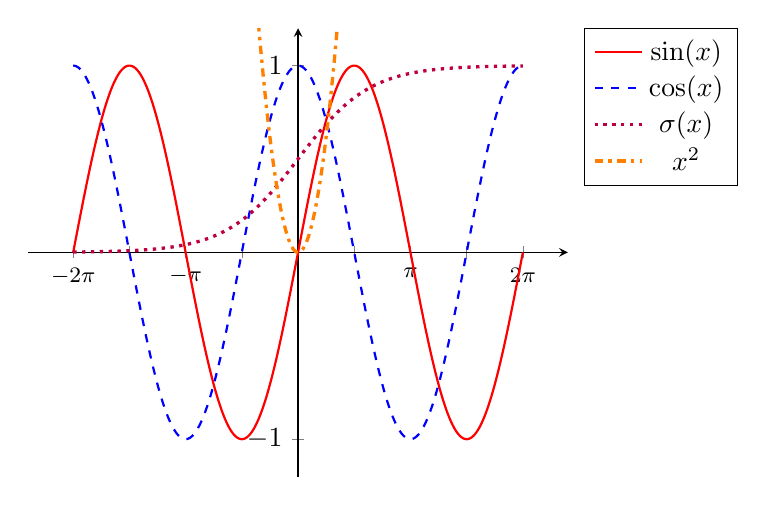
\begin{tikzpicture}
    \begin{axis}[
        legend pos=outer north east,
        xtick={-2*pi, -(3/2)*pi, -pi, -(1/2)*pi, (1/2)*pi, pi, (3/2)*pi, 2*pi},
        %        xtick={-6.28318, -4.7123889, -3.14159, -1.5708, 1.5708, 3.14159, 4.7123889, 6.28318},
        xticklabel style={font=\footnotesize,fill=white},
        xticklabels={$-2\pi$,,$-\pi$,,,$\pi$,,$2\pi$},
        ytick={-1,1},
        axis lines=middle,
        domain=-2*pi:2*pi,
        samples=501,
        enlargelimits=true,
        ymax=1, ymin=-1,
        ]
    \addplot[thick, solid, red] {sin(deg(x))};
    \addplot[thick, dashed,blue] {cos(deg(x))};
    \addplot[very thick, dotted,purple] {1/(1+ exp(-x))};
    \addplot[very thick, dashdotted,orange] {x^2};
    \legend{$\sin(x)$,$\cos(x)$,$\sigma(x)$,$x^2$}
    \end{axis}
\end{tikzpicture}
\end{minipage}

{%
    \checkboxchar{$\Box$} \checkedchar{$\blacksquare$} % change checkbox style locally
    \begin{checkboxes}
     \choice $f(x) = \sin(x)$
     \choice $f(x) = \cos(x)$
     \choice $f(x) = \sigma(x)$
     \choice $f(x) = x^2$
     \choice None of the above
    \end{checkboxes}
}
\begin{soln}
    B, D
\end{soln}
\begin{qauthor}
    Alex, Convert linearly inseparable dataset to a linearly separable dataset in higher
dimensions. Matt, added plot.
\end{qauthor}

\begin{qtester}
I like this question.
\end{qtester}


\part Neural creates a linear regression model $M_1$ for work, but his boss Markov tells him that $M_1$ uses too many features 
% COMMENTING OUT TO NOT GIVE THINGS AWAY: 
% (i.e., has too many features with nonzero coefficients) 
to be easily explained. He decides to use ridge regression (L2 regularization) to identify and remove irrelevant features. Neural trains a new model using ridge regression, then removes every feature with a weight of exactly $0$ from his model---he dubs the result $M_2$. However, $M_2$ still uses the same number of features as $M_1$ after this process (i.e., no features were removed).

\begin{subparts}
    \subpart[1] \textbf{Short answer:} Explain why the feature removal process was not effective at getting rid of features.
    \fillwithlines{6em}
    \begin{soln}
    L2 penalty doesn't push many parameters to $0$, can leave them at very small values. They won't get removed in step 2.
    \end{soln}

    \subpart[1] \textbf{Short answer:} Describe an alternative method of feature selection using $L2$ regularization that would reliably get rid of some features.
    \fillwithlines{6em}
    \begin{soln}
        L2 but remove the $k$ features with smallest weight, instead of only exactly 0
    \end{soln}

    \subpart[1] \textbf{Short answer:} Describe a method of feature selection via another form of regularization that Neural could use.
    \fillwithlines{6em}
    \begin{soln}
    LASSO
    \end{soln}
\end{subparts}
    \begin{qauthor}
    Abhi, Use feature selection techniques to identify and remove irrelevant features
    \end{qauthor}
\begin{qtester}
I like this question. I suspect we will get some creative answers about why it was not effective, but that's probably ok.
\end{qtester}     
\end{comment}
\end{parts}
\clearpage
\sectionquestion{Logistic Regression}

\begin{parts}


\part Consider a binary classification problem over labels $y \in \{0,1\}$. In binary logistic regression, we use the sigmoid $\sigma(a)$ function to map real valued scalars to probabilities between 0 and 1. Now suppose we define a new model \emph{binary tanh regression} for the same task by swapping out the sigmoid function for another one: 
\begin{align*}
    p(y=1|\xv,\theta) = \frac{\tanh(\theta^T\xv)+1}{2} 
    \text{ where } 
    \tanh(a) = \frac{\exp(a)-\exp(-a)}{\exp(a)+\exp(-a)}
\end{align*}
A convenient property you may use is that $\tanh(a) = n\sigma(na)-1$ for $n=2$.
\begin{subparts}
    % \subpart[2]{It can be shown that $\tanh(a) = n\sigma(na)-1$ for some integer $n$. What is the value of $n$?} 
    % \begin{tcolorbox}[fit,height=1.5cm, width=4cm, blank, borderline={1pt}{-2pt}]
    %             %solution
    % \end{tcolorbox} 
    % \begin{soln}
    %     Equating both sides we get:
    %     \begin{equation}
    %          \frac{2\exp(x)}{\exp(x)+\exp(-x)} = \frac{2}{1+\exp(-2x)} = \frac{n}{1+\exp(-nx)}
    %     \end{equation}
    %     Thus we get $n=2$
    % \end{soln}
    
    \subpart[2] \textbf{Short answer:} For a single example $(\xv^{(i)},y^{(i)})$, what is the likelihood of this data point under this new model? Your answer should be in terms of $\theta,\sigma,\xv^{(i)},y^{(i)}$, it should not include $n$ or $\tanh$. \textit{For full credit, you must define a single expression without cases. }
    \begin{tcolorbox}[fit,height=2cm, width=15cm, blank, borderline={1pt}{-2pt}]
                %solution
    \end{tcolorbox} 
    \begin{soln}
        \begin{equation}
            L = p(y^{(i)}=1|x^{(i)},\theta)^{y^{(i)}} (1-p(y^{(i)}=1|x^{(i)},\theta))^{1-y^{(i)}}
        \end{equation}
        \begin{equation}
            L = \sigma(2\theta^T x^{(i)})^{y^{(i)}} (1-\sigma(2\theta^T x^{(i)}))^{1-y^{(i)}}
        \end{equation}
    \end{soln}
    
    \subpart[2] \textbf{Short answer:} What is the negative log likelihood for this one example $(\xv^{(i)},y^{(i)})$? Your answer should be in terms of $\theta,\sigma,\xv^{(i)},y^{(i)}$, it should not include $n$ or $\tanh$. 
    \textit{For full credit, you must define a single expression without cases. }
    \begin{tcolorbox}[fit,height=2cm, width=15cm, blank, borderline={1pt}{-2pt}]
                %solution
    \end{tcolorbox} 
    \begin{soln}
        \begin{equation}
            -\log L = -y_i \log(\sigma(2\thetav^T\xv_i)) - (1-y_i)(\log(1-\sigma(2\thetav^T\xv_i)))
        \end{equation}
    \end{soln}

    % SKIPPED FOR TIME:
    %
    % \subpart[3] \textbf{Short answer:} Let $J^{(i)}(\theta)$ denote the negative log likelihood for this one example. What is $\frac{\partial J^{(i)}(\theta)}{\partial \theta_j}$? Your answer should be in terms of $\theta,\sigma,x^{(i)},y^{(i)}$, it should not include $n$ or $\tanh$. \textit{Hint:} Some useful derivatives: $\frac{\partial \sigma(a)}{\partial a} = \sigma(a)(1 - \sigma(a))$ and $\frac{\partial \log(b)}{\partial b} = \frac{1}{b}$.
    % \begin{tcolorbox}[fit,height=4cm, width=15cm, blank, borderline={1pt}{-2pt}]
    %             %solution
    % \end{tcolorbox} 
    % \begin{soln}
    %     \begin{align*}
    %         \frac{\partial J^{(i)}(\theta)}{\partial \theta_j} 
    %         &= \frac{\partial}{\partial \theta_j}\left(  -y_i \log(\sigma(2\thetav^T\xv_i)) - (1-y_i)(\log(1-\sigma(2\thetav^T\xv_i))) \right) \\
    %         &= \frac{\partial}{\partial \theta_j}\left(  -y_i \log(\sigma(2\thetav^T\xv_i)) - (1-y_i)(\log(1-\sigma(2\thetav^T\xv_i))) \right) \\
    %         &= 2(\sigma(2 \thetav^T \xv^{(i)}) - y^{(i)}) x_j^{(i)} 
    %     \end{align*}
    % \end{soln}

    \subpart[2] \textbf{Short answer:} Now consider a dataset of $N$ points $\Dc = \{ (\xv^{(i)},y^{(i)}) \}_{i=1}^N$. Write the update rule for the vector $\thetav$ using gradient descent assuming the objective function to be the average negative log likelihood over the $N$ points. Take the learning rate to be $\eta$. Your answer should be in terms of $\theta,\sigma,\xv^{(i)},y^{(i)}$,$N$,$\eta$, it should not include $n$ or $\tanh$---and it must include the term $\nabla J^{(i)}(\thetav)$ where $J^{(i)}(\theta)$ denotes the negative log likelihood for the $i$th example (i.e. we don't want you to do any calculus here). 
    \begin{tcolorbox}[fit,height=2cm, width=15cm, blank, borderline={1pt}{-2pt}]
                %solution
    \end{tcolorbox} 
    \begin{soln}
        \begin{equation}
            %\theta_j \leftarrow \theta_j - \eta \frac{1}{N} \sum_{i=1}^N 2(\sigma(2 \theta^T x^{(i)}) - y^{(i)}) x_j^{(i)} 
            %\thetav \leftarrow \thetav - \eta \frac{1}{N} \sum_{i=1}^N 2(\sigma(2 \thetav^T \xv^{(i)}) - y^{(i)}) \xv^{(i)} 
            \thetav \leftarrow \thetav - \eta \frac{1}{N} \sum_{i=1}^N \nabla J^{(i)}(\thetav)
        \end{equation}
    \end{soln}
    
\end{subparts}
    \begin{qauthor}
    Pranit, Logistic Regression, Given a discriminative probabilistic model, derive the conditional log-likelihood
    (adapted by Matt)
    \end{qauthor}

 \clearpage
\part Consider the test dataset below for binary classification containing five points, two are labeled $y = +1$ (indicated by a square $\blacksquare$), two are labeled $y = -1$ (indicated by a triangle $\blacktriangle$), and one has unknown label $y \in \{+1, -1\}$ (indicated by a circle $\bullet$, $\xv^{(5)} = (1.0,0.5)$). 
%
We employ a logistic regression model to classify these points according to a modified decision rule: if $\sigma(w^Tx+b) \ge t$ then $y=+1$, otherwise $y=-1$, where the threshold $t \in [0,1]$. Assume that $w=[1,-1]^T$, $b=0$. 
%
Furthermore, you have access to a plot depicting the accuracy of this model across the five points as the threshold $t$ is adjusted. 
%Hint: $\sigma(0.5) = 0.62$, $\sigma(1) = 0.73$, and $\sigma(x)+\sigma(-x)=1$. 
%Answer the questions given below based on this information. 

\begin{minipage}{0.5\linewidth}
    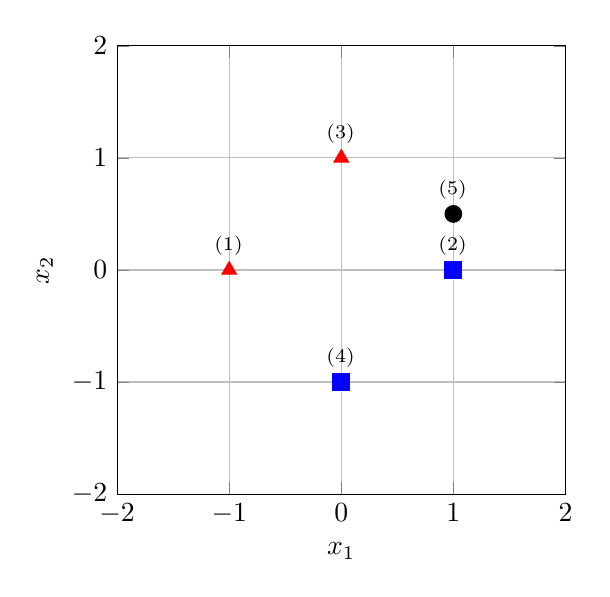
\begin{tikzpicture}
    \begin{axis}[
        scale=1, axis equal image, mark options={scale=1.5},
        xmin=-2, xmax=2, xtick={-2,...,2},
        ymin=-2, ymax=2, ytick={-2,...,2},
        samples=50, grid=major, xlabel=$x_1$, ylabel=$x_2$]]
        \addplot [
            scatter,
            only marks,
            point meta=explicit symbolic,
            scatter/classes={
                a={mark=square*,blue},
                b={mark=triangle*,red},
                c={mark=*,black}
            },
            nodes near coords*={$\xv^{(\pgfmathprintnumber[frac]\myvalue)}$},
            visualization depends on={\thisrow{myvalue} \as \myvalue},
        ] table [meta=label] {
            x y label myvalue
            -1 0 b 1
            1 0 a 2
            0 1 b 3
            0 -1 a 4
            1 0.5 c 5
        };
        %\addplot[ultra thick, color=green] coordinates { (-2,-2) (2,2) };
        %\draw[->, >=stealth, ultra thick, color=green] (axis cs:0,0) -- (axis cs:1,-1);
    \end{axis}
    \end{tikzpicture} 
\end{minipage}
\begin{minipage}{0.5\linewidth}
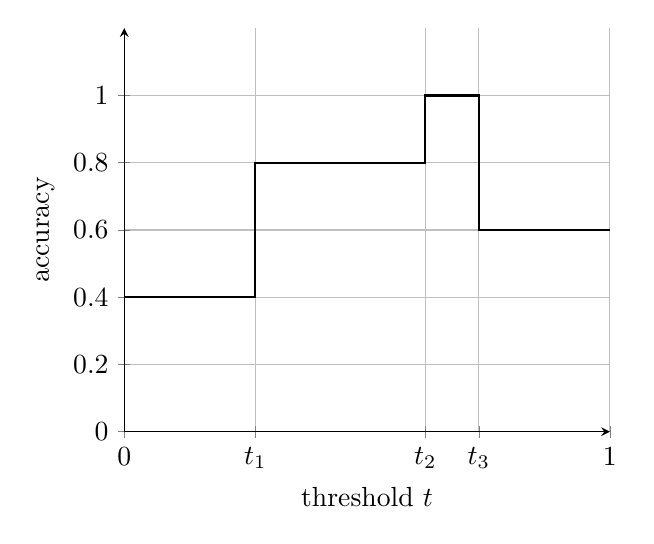
\begin{tikzpicture}
\begin{axis}[
    scale=0.9,
    axis lines = left,
    xlabel = threshold $t$,
    ylabel = {accuracy},
    ymin=0, ymax=1.2,
    xmin=0,xmax=1,
    xtick={0,0.27,0.62,0.73,1},
    xticklabels={0,$t_1$, $t_2$, $t_3$,1},
    ytick={0,0.2,0.4,0.6,0.8,1},
    % xtick={0,1},
    % ytick={0,0.2,0.4,0.6,0.8,1},
    % xticklabels={0,$t_1$,$t_2$,$t_3$},
    % yticklabels={0,0.2,0.4,0.6,0.8,1},
    grid=both,
    ]
    \addplot[const plot, no marks, thick] coordinates {
        (0,0.4) (0.27,0.8) (0.62,1) (0.73,0.6) (1,0.6)
    };

\end{axis}
\end{tikzpicture}
\end{minipage}

\begin{subparts}
    \subpart[1] What is the label of point $x^{(5)}?$ 
    \begin{checkboxes}
        \choice  $y^{(5)} = +1$
        \choice  $y^{(5)} = -1$
    \end{checkboxes}
    \begin{soln}
        Label of $x^{(5)} = -1$\\ 
        From either threshold = 0 or threshold =1, we can see that $x^{(5)}$ will be -1. 
    \end{soln}
    
    \subpart[2] What is the value $a_2$ such that $\sigma(a_2) = t_2$?
    \begin{tcolorbox}[fit,height=1.5cm, width=6cm, blank, borderline={1pt}{-2pt}]
                %solution
    \end{tcolorbox}
    \begin{soln}
        $a_2 = 0.5$ and $t_2 = 0.62$ \\ 
        From either threshold = 0 or threshold =1, we can see that $x^{(5)}$ will be -1. Now, we can see that the accuracy can be 1 only if $x^{(5)}$ is classified correctly.  i.e. when $ \sigma(0.5) \le t \le \sigma(1)$ which gives us the answer.  \\
        Give partial credit for $t \in $
    \end{soln}

    \subpart[2] What is the value $a_3$ such that $\sigma(a_3) = t_3$?
    \begin{tcolorbox}[fit,height=1.5cm, width=6cm, blank, borderline={1pt}{-2pt}]
                %solution
    \end{tcolorbox}
    \begin{soln}
        $a_3 = 1.0$ and $t_3 = 0.73$ \\
    \end{soln}

    \end{subparts}
    \begin{qauthor}
    Pranit, Logistic Regression (LO:  Implement logistic regression for binary or multiclass classification)
    (adapted by Matt)
    \end{qauthor}
    
\begin{comment} 
\part \textbf{Matching:} Consider the three algorithms and four update rules shown below. For any algorithm that requires it, assume we are using a fixed learning rate $\gamma$. Match each algorithm to its update rule. It is possible that multiple algorithms may match to the same rule. Assume the bias term is folded into $\thetav$.
    
    \begin{table}[H]
    \vspace{-.5em}
        \begin{subtable}{.5\linewidth}
            \centering
            \begin{tabular}{p{0.7\linewidth}}
                \toprule
                \textbf{Algorithms:} \\
                \midrule
                (A) SGD for Logistic Regression 
                \newline \hspace*{2em} $\displaystyle h_{\thetav}(\xv) = p(y=1|x)$ \\
                \midrule
                %
                (B) SGD for Linear Regressions
                \newline \hspace*{2em}$\displaystyle h_{\thetav}(\xv) = \thetav^T \xv$ \\
                \midrule
                %
                (C) Perceptron 
                \newline \hspace*{2em} $\displaystyle h_{\thetav}(\xv) = \text{sign}(\thetav^T \xv)$ \\
                 \hspace*{2em} where $\text{sign}(\cdot) \in \{-1, +1\}$ \\
                \bottomrule
              \end{tabular}
        \end{subtable}
        \begin{subtable}{.5\linewidth}
            \centering
            \begin{tabular}{l}
                \toprule
                \textbf{Update Rules:} Each is of the form \\
                $\thetav \leftarrow \thetav - \gv$ where \\
                \midrule
                (1) $\displaystyle g_k = (h_{\thetav}(\xv^{(i)}) - y^{(i)})$\\
                \midrule
                (2) $\displaystyle g_k =  \gamma (h_{\thetav}(\xv^{(i)}) - y^{(i)}) x_k^{(i)}$\\
                \midrule
                %
                %
                (3) $\displaystyle g_k = \frac{1}{1 + \exp \gamma (h_{\thetav}(\xv^{(i)}) - y^{(i)}) }$\\
                \midrule
                %
                (4) $\displaystyle g_k =  \gamma  \frac{1}{N} \sum_{i=1}^N (h_{\thetav}(\xv^{(i)}) - y^{(i)}) x_k^{(i)}$\\
                \bottomrule
            \end{tabular}
      \end{subtable}
      
    \vspace{-.5em}
    \end{table}
    
    {\small 
    \begin{subparts}
        \subpart[1] Which of the following is the correct update rule for Algorithm A?
        \begin{checkboxes}
        \choice Update Rule (1)
        \choice Update Rule (2)
        \choice Update Rule (3)
        \choice Update Rule (4)
        \end{checkboxes}
        \subpart[1] Which of the following is the correct update rule for Algorithm B? 
        \begin{checkboxes}
        \choice Update Rule (1)
        \choice Update Rule (2)
        \choice Update Rule (3)
        \choice Update Rule (4)
        \end{checkboxes}
        \subpart[1] Which of the following is the correct update rule for Algorithm C? 
        \begin{checkboxes}
        \choice Update Rule (1)
        \choice Update Rule (2)
        \choice Update Rule (3)
        \choice Update Rule (4)
        \end{checkboxes}
    \end{subparts}
    }
    \begin{soln}
        \begin{enumerate}
        \item (2)
        \item (2)
        \item (2)
    \end{enumerate}
    \end{soln}
    
    \begin{qauthor}
    Tara (Matt adapted back into a matching question to reduce reading time. Similar to S19 version.)
    \end{qauthor}

\clearpage

\newcommand{\NarName}{Graddyant}
\part \NarName{} the Narwhal\texttrademark\,\textit{really} doesn't like the sigmoid in binary logistic regression and proposes the following binary classification model using softmax instead. Let the input to the model be $\xv \in \mathbb{R}^m$, let the label be $y \in \{ 0, 1 \}$, and let the model weights be $\Av \in \mathbb{R}^{2 \times m}$, where $\Av_1, \Av_2 \in \mathbb{R}^m$ refer to the first and second rows of $\Av$.
\begin{align*}
\zv &= \Av \xv = [\Av_1 \xv, \Av_2 \xv]^T \\
\hv &= \text{softmax}(\zv) = \bigg[ \frac{e^{z_1}}{e^{z_1} + e^{z_2}}, \frac{e^{z_2}}{e^{z_1} + e^{z_2}} \bigg]^T
\end{align*}
Under \NarName{}'s formulation, $h_1$ represents $P(y = 0 \,|\, \xv)$ and $h_2$ represents $P(y = 1 \,|\, \xv)$.
\begin{subparts}
    \subpart \textbf{Fill in the blanks:} Fill in the blanks in the expression below for the log likelihood of a single example $(\xv, y)$. Your answers should be in terms of $\Av_1, \Av_2$ and $\xv$.
    
    \textit{(Hint: Recall for a sample $b$ of a Bernoulli random variable $B$ with parameter $\phi$, we write the likelihood of $b$ as $\phi^b(1-\phi)^{(1-b)}$.)}
    \begin{align*}
        (\blankforFITB{2em}{i.}) \cdot y + (\blankforFITB{2em}{ii.}) \cdot (1 - y) - \log(e^{z_1} + e^{z_2})
    \end{align*}
    \begin{subsubparts}
    \subsubpart[1]
    \begin{tcolorbox}[fit,height=1.5cm, width=6cm, blank, borderline={1pt}{-2pt}, nobeforeafter]
                %solution
    \end{tcolorbox}
    \subsubpart[1]
    \begin{tcolorbox}[fit,height=1.5cm, width=6cm, blank, borderline={1pt}{-2pt}, nobeforeafter]
                %solution
    \end{tcolorbox}
    \end{subsubparts}
    \begin{soln}
    \begin{align*}
        \ell(\Av) &= y \log h_2 + (1-y) \log h_1 \\
        &= y z_2 + (1-y) z_1 - \log(e^{z_1} + e^{z_2}) \\
        &= A_2 x \cdot y + A_1 x \cdot (1-y) - \log(e^{z_1} + e^{z_2})
    \end{align*}
    \end{soln}   
    \begin{qtester}
    We should maybe put a,b on the blank lines and label the corresponding boxes.
    \end{qtester}
    \subpart[1] \textbf{Fill in the blank:} Fill in the decision rule of the Bayes optimal classifier, assuming all mistakes incur a loss of 1. Your answer should be in terms of $z_1$ and $z_2$. If there are ties, you may break them arbitrarily.
    \begin{align*}
        \hat{y} = \begin{cases} 1 & \text{if } \blankforFITB{2em}{} \\ 0 & \text{otherwise} \end{cases}
    \end{align*}
    \begin{tcolorbox}[fit,height=1.5cm, width=6cm, blank, borderline={1pt}{-2pt}, nobeforeafter]
                %solution
    \end{tcolorbox}
    
    \begin{soln}
        $z_2 \geq z_1$ or $z_2 > z_1$ or equivalent
    \end{soln}

\clearpage

    \subpart[3] \textbf{Proof:} Neural claims that \NarName{}'s model yields exactly the same decision boundary as a log regression model $p(y=1 \mid \xv) = \sigma(\thetav^T\xv)$ with weights $\thetav = \Av_2^T - \Av_1^T$. Is Neural right? If yes, show that the decision boundaries are mathematically equivalent. If not, give a specific weight matrix $\Av$ and input $\xv$ that contradicts Neural's statement.
    
    \begin{tcolorbox}[fit,height=7cm, width=15cm, blank, borderline={1pt}{-2pt}]
    %solution
    \end{tcolorbox}

    \begin{soln}
        The decision boundary of log regression is $\sigma(\theta^T x) \geq 0.5 \iff \theta^T x \geq 0 \iff (\Av_2 - \Av_1) x \geq 0 \iff \Av_2 x \geq \Av_1 x \iff z_2 \geq z_1$.
    \end{soln}

    % Matt: Commenting out this subpart as it's not needed here.
    %
    % \subpart[1] \textbf{Numerical answer;} In terms of $m$ (recall that $\xv \in \mathbb{R}^m$), what is the VC dimension of Gradient's model?
    %
    % \begin{tcolorbox}[fit,height=1cm, width=4cm, blank, borderline={1pt}{-2pt}, nobeforeafter]
    % \end{tcolorbox}
    %
    % \begin{soln}
    %     $m$ since we don't have a bias
    % \end{soln}
\end{subparts}
\begin{qauthor}
    Alex \\
    Given a discriminative probabilistic model, derive the conditional log-likelihood, its
gradient, and the corresponding Bayes Classifier \\
    Technically we don't have a learning objective for VC dimension - is it still fair game?
\end{qauthor}

\begin{qtester}
I think VC dimension would be fair game, but we should check with Matt. I also wonder if this question is a bit long with the amount of reading along with a derivation. 
\end{qtester}
\begin{qauthor}
    I don't mind deleting some parts of the question, the main reason I wrote it was for the decision boundary question in part (c).
\end{qauthor}


\part Suppose we are performing logistic regression, with $p(y=1|\xv,\thetav) = \sigma(\thetav^T \xv)$ (no intercept term). Normally, the decision rule for classifying a data point as a positive is $\sigma(\thetav^T \xv) \ge 0.5$, and we say that the \textit{threshold of classification} is 0.5 in this case. 
Suppose we instead use a \emph{modified} decision rule that classifies as positive when $p(y=1|\xv,\thetav) \ge t p(y=0|\xv,\thetav)$ where $t$ is a scalar such that $ t > 0 $. 
\begin{subparts}
    \subpart[2] \textbf{Derivation:} What is the \emph{modified} threshold of classification in terms of $t$? Show your work in the box below and circle your final answer for the threshold.
   
    
    \begin{tcolorbox}[fit,height=7cm, width=15cm, blank, borderline={1pt}{-2pt}, nobeforeafter]
    \end{tcolorbox}

    \begin{soln}
    \begin{equation}
         p(y=1|x,\theta) \ge tp(y=0|x,\theta)
    \end{equation}
    \begin{equation}
        p(y=1|x,\theta) \ge t(1-p(y=1|x,\theta))
    \end{equation}
    \begin{equation}
        p(y=1|x,\theta) \ge \frac{t}{t+1} \implies \sigma(\theta^Tx) \ge \frac{t}{t+1}
    \end{equation}

    \end{soln}
    \begin{qauthor}
    Pranit
    \end{qauthor}
    \begin{qtester}
    I like this, but it seems a bit difficult for the 601 exam. we would also need to allow more space for student work. 
    \end{qtester}

    % Matt: removed b/c this part is out of scope.
    % 
    % \subpart[1] \textbf{Fill in the blank:} Let the modified decision boundary be $\theta^Tx + f(t) = 0$, where $f(t)$ is a function of $t$. What is $f(t)$? Is $f(t)$ convex?

    % \begin{tcolorbox}[fit,height=1cm, width=4cm, blank, borderline={1pt}{-2pt}, nobeforeafter]
    % \end{tcolorbox}

    % \begin{soln}
    % \begin{equation}
    %     \sigma(\theta^Tx) = \frac{t}{t+1}
    % \end{equation}
    % \begin{equation}
    %     \frac{1}{1+\exp(-\theta^Tx)} = \frac{t}{t+1}
    % \end{equation}
    % \begin{equation}
    %     t + 1 = t + t\exp(-\theta^Tx)
    % \end{equation}
    % \begin{equation}
    %     \theta^Tx - \log(t) = 0 \implies f(t) = -\log(t)
    % \end{equation}
    % Yes $f(t)$ is convex. 
    % \end{soln}

    % \begin{qauthor}
    % Pranit
    % \end{qauthor}
    % \begin{qtester}
    % This seems a bit difficult for the 601 exam. we would also need to allow more space for student work. 
    % \end{qtester}

\clearpage

\subpart[2] \textbf{Select all that apply:} Which of the following are true of the modified decision rule?
    {%
    \checkboxchar{$\Box$} \checkedchar{$\blacksquare$} % change checkbox style locally
    \begin{checkboxes}
     \choice For lower values of t (close to 0) there will be very few false negative predictions by the modified decision rule. (A false negative is when we mistakenly predict negative.)
     \choice For very large values of t ($>> 1$) there will be a large number of false positive predictions by the modified decision rule. (A false positive is when we mistakenly predict positive.)
     \choice Using $t=\frac{1}{2}$ returns the standard logistic regression model. 
     \choice The modified decision boundary will only be linear if $t > \frac{1}{2}$.
     \choice None of the above
    \end{checkboxes}
    }
    \begin{soln}
    A \\ 
    A is true because lower values of $t$ will make the model classify almost all points as positives, and hence the recall will be very high with low false negatives. \\
    B is false because large values of $t$ means that very few points will be classified as positives, and thus the precision will be very high. \\ 
    C is false because $t=1$ returns the usual logistic regression model \\ 
    D is false because the decision boundary is always linear
    \end{soln}

    \begin{qauthor}
    Pranit, Prove that the decision boundary of binary logistic regression is linear, 
    \end{qauthor}

\end{subparts}
\end{comment}

\end{parts}
\clearpage
\sectionquestion{Neural Networks \& Backpropagation}

\begin{parts}


% Question 3 and 6 merged into one
\part Consider the neural network with $1$ hidden layer shown below for a binary classification problem, where $\xv \in \Rb^3$ is the input feature vector and $\yv \in \Rb^2$ is a one-hot vector representing the correct class. Note: this network does not contain bias terms.

%
\begin{minipage}{0.5\linewidth}
%\begin{figure}[h]
    \def\distH{2.5cm}
    \def\distHTwo{2.0cm}
    \def\distHThree{0.3cm}
    \def\distV{0.6cm}
    \def\distVTwo{0.3cm}
    \centering
    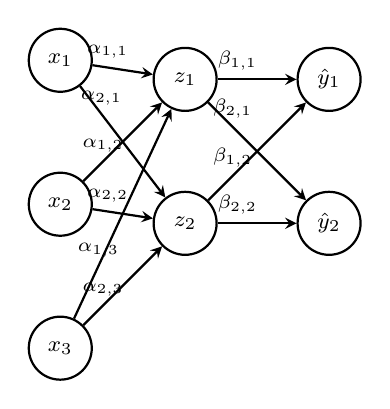
\begin{tikzpicture}[
        > = stealth, % arrow head style
        shorten > = 0pt, % don't touch arrow head to node
        auto,
        % node distance = 2.5cm, % distance between nodes
        thick % line style
    ]\footnotesize
    \tikzstyle{every state}=[
        draw = black,
        thick,
        fill = white,
        minimum size = 0.8cm,
    ]
    \node[state] (X1){$x_1$};
    \node[state] (X2) [below = \distV of X1] {$x_2$};
    \node[state] (X3) [below = \distV of X2] {$x_3$};
    \node[state] (Z1) [above right = \distVTwo and \distH of X2] {$z_1$};
    \node[state] (Z2) [below = \distV of Z1] {$z_2$};
    \node[state] (y1) [right = \distHTwo of Z1] {$\hat{y}_1$};
    \node[state] (y2) [right = \distHTwo of Z2] {$\hat{y}_2$};

    \path[->] (X1) edge node  [above, near start, font=\scriptsize]{$\alpha_{1,1}$} (Z1);
    \path[->] (X1) edge node [above, near start, font=\scriptsize]{$\alpha_{2,1}$} (Z2);
    \path[->] (X2) edge node [above, near start, font=\scriptsize]{$\alpha_{1,2}$} (Z1);
    \path[->] (X2) edge node [above, near start, font=\scriptsize]{$\alpha_{2,2}$} (Z2);
    \path[->] (X3) edge node [above, near start, font=\scriptsize]{$\alpha_{1,3}$} (Z1);
    \path[->] (X3) edge node [above, near start, font=\scriptsize]{$\alpha_{2,3}$} (Z2);
    \path[->] (Z1) edge node [above,  near start, font=\scriptsize] {$\beta_{1,1}$} (y1);
    \path[->] (Z2) edge node [above, near start,  font=\scriptsize]{$\beta_{1,2}$} (y1);
    \path[->] (Z1) edge node [above, near start,  font=\scriptsize]{$\beta_{2,1}$} (y2);
    \path[->] (Z2) edge node [above,  near start, font=\scriptsize]{$\beta_{2,2}$} (y2);
    \end{tikzpicture}
    %\caption{neural network diagram}
    %\label{fig:nn_graph}
%\end{figure}
\end{minipage}
\begin{minipage}{0.5\linewidth}
\begin{align*}
    %&\mathbf{x} = [x_1, x_2, x_3]^T\\
    &a_1 = \alpha_{1,1} x_1 + \alpha_{1,2} x_2 + \alpha_{1,3} x_3 \\
    &a_2 = \alpha_{2,1} x_1 + \alpha_{2,2} x_2 + \alpha_{2,3} x_3 \\
    %&a_j = \sum_{i=1}^{3} \alpha_{j, i} \cdot x_i , \,\,  \forall j \in \{1, 2\}\\
    &z_j = \max(0, a_i) ,\,\,  \forall j \in \{1, 2\}\\
    &b_1 = \beta_{1,1} z_1 + \beta_{1,2} z_2 \\
    &b_2 = \beta_{2,1} z_1 + \beta_{2,2} z_2 \\
    %&b_k = \sum_{j=1}^{2} \beta_{k, j} \cdot z_j ,\,\, \forall k \in \{1, 2\}\\
    &\hat{y}_k = \exp(b_k)/(\exp(b_1)+\exp(b_2)) ,\,\,  \forall k \in \{1, 2\}\\
    &\ell = - \sum_{k=1}^2 y_k \log(\hat{y}_k)
\end{align*}
\end{minipage}

\begin{qauthor}
    Zoe Xu; Implement a feed-forward neural network; Construct a computation graph for a neural network, identifying all the given and intermediate quantities that are relevant.
\end{qauthor}

\begin{subparts}


\subpart[2] \textbf{Numerical answer:} 
    Given $\xv = [1, 2, 0]^T$, $\alpha_{j,i} = 1\,\,\forall j,i$, $\beta_{k,j} = 1\,\, \forall k,j$. Compute $b_2$. (You should ignore these numerical values for all subsequent questions.)

    \begin{tcolorbox}[fit,height=1cm, width=2cm, blank, borderline={1pt}{-2pt}]
    %solution
    \end{tcolorbox}
    \begin{soln}
    $b_2 = 6$
    \end{soln}

\subpart[2] \textbf{Math:} What is the chain of partial derivatives needed by symbolic differentiation to calculate the derivative $\frac{\partial \ell}{\partial\alpha_{j,i}}$ for $i \in \{1, 2, 3\}$ and $j \in \{1, 2\}$?

    Your answer should be in the form: 
    $\frac{\partial \ell}{\partial \alpha_{j,i}} = \frac{\partial ?}{\partial ?} \frac{\partial ?}{\partial ?} \dots$
    Make sure each partial derivative $\frac{\partial ?}{\partial ?}$ in your answer cannot be decomposed further into simpler partial derivatives. You may intersperse summations between the $\frac{\partial ?}{\partial ?}$ terms.

    \begin{tcolorbox}[fit,height=3cm, width=15cm, blank, borderline={1pt}{-2pt},nobeforeafter]
    \begin{soln}
        $\frac{\partial \ell}{\partial \alpha_{j,i}} = \sum_{k=1}^2 
        \frac{\partial \ell}{\partial \hat{y}_k} 
        \frac{\partial \hat{y}_k}{\partial b_k}
        \frac{\partial b_k}{\partial z_j} 
        \frac{\partial z_j}{\partial a_j} 
        \frac{\partial a_j}{\partial \alpha_{j,i}}$ \newline \newline
        $\frac{\partial \ell}{\partial \alpha_{j,i}} = \sum_{k=1}^2 
        \frac{\partial \ell}{\partial \hat{y}_k}\sum_{n=1}^2 
        \frac{\partial \hat{y}_k}{\partial b_n} 
        \frac{\partial b_n}{\partial z_j} 
        \frac{\partial z_j}{\partial a_j} 
        \frac{\partial a_j}{\partial \alpha_{j,i}}$
    \end{soln}
    \end{tcolorbox}
    \begin{qauthor}
        Shivi, Instantiate the backpropagation algorithm for a neural network
        (Adapted by Matt)
    \end{qauthor}

\clearpage
\subpart[3] \textbf{Math:} What is the sequence of partial derivatives \emph{stored} by the backpropagation algorithm before it computes \textit{any} of the derivatives $\frac{\partial \ell}{\partial\alpha_{j,i}}$ for $i \in \{1, 2, 3\}$ and $j \in \{1, 2\}$?

    Your answer should be in the form of a list: 
    $[\frac{\partial ?}{\partial ?}, \frac{\partial ?}{\partial ?}, \dots , \frac{\partial ?}{\partial ?}]$, such that each item is stored by backpropagation before all items that appear after it in the list.
    Make sure each partial derivative $\frac{\partial ?}{\partial ?}$ in your answer cannot be decomposed further into simpler partial derivatives. 
    
    \begin{tcolorbox}[fit,height=3cm, width=15cm, blank, borderline={1pt}{-2pt},nobeforeafter]
    \begin{soln}
        $[
        \frac{\partial \ell}{\partial \hat{y}_1}, 
        \frac{\partial \ell}{\partial \hat{y}_2}, 
        \frac{\partial \ell}{\partial b_1},
        \frac{\partial \ell}{\partial b_2},
        \frac{\partial \ell}{\partial z_1}, 
        \frac{\partial \ell}{\partial z_2},
        \frac{\partial \ell}{\partial a_1}, 
        \frac{\partial \ell}{\partial a_2}
        ]
        $
    \end{soln}
    \end{tcolorbox}
    \begin{qauthor}   Matt    \end{qauthor}
    
\subpart[2] \textbf{Math:} Write an expression for how backpropagaion computes $\frac{\partial \ell}{\partial\alpha_{j,i}}$ for $i \in \{1, 2, 3\}$ and $j \in \{1, 2\}$, after the algorithm has stored all the partial derivatives in your list from the previous question.

    Your answer should be in the form: 
    $\frac{\partial \ell}{\partial \alpha_{j,i}} = \frac{\partial ?}{\partial ?} \frac{\partial ?}{\partial ?} \dots$
%Your answer should be a mathematical expression containing only variables introduced in the problem introduction, along with necessary constants, mathematical notation and/or subscripts.
    
    \begin{tcolorbox}[fit,height=3cm, width=15cm, blank, borderline={1pt}{-2pt},nobeforeafter]
    \begin{soln}
        $\frac{\partial \ell}{\partial\alpha_{j,i}} =
        \frac{\partial \ell}{\partial a_j}
        \frac{\partial a_j}{\partial \alpha_{j,i}}
        $
    \end{soln}
    \end{tcolorbox}
    \begin{qauthor}   Matt    \end{qauthor}

    
    
\subpart[3] Complete the stochastic gradient descent implementation below in order to update $\alpha_{j,i}$ and $\beta_{k,j}$. (You may use $\frac{\partial \ell}{\partial\alpha_{j,i}}$ and/or $\frac{\partial \ell}{\partial\beta_{k,j}}$, if needed.)

    \begin{tcolorbox}[height=7.5cm, width=15cm, blank, borderline={1pt}{-2pt},nobeforeafter]
    %\begin{algorithm}
    %\caption{Stochastic Gradient Descent for One-Hidden-Layer Neural Network}
    \begin{algorithmic}
    \State Initialize weights \(\alpha_{j,i}\) and \(\beta_{k,j}\) randomly
    \State Choose learning rate \(\eta\)
    \For{each epoch}
        \For{each training example \((\xv, \yv)\)}
            \State // Compute gradients
            \State 
            \State 
            \State
            \State
            \State // Update weights
            \State 
            \State 
            \State
            \State
        \EndFor
    \EndFor
    \end{algorithmic}
    %\end{algorithm}
    \end{tcolorbox}
    
    \begin{soln}
    %\begin{algorithm}
    %\caption{Stochastic Gradient Descent for One-Hidden-Layer Neural Network}
    \begin{algorithmic}
    \State Initialize weights \(\alpha_{j,i}\) and \(\beta_{k,j}\) randomly
    \State Choose learning rate \(\eta\)
    \For{each epoch}
        \For{each training example \((\xv, \yv)\)}
            \State // Compute gradients
            \State $g_{\beta_{k,j}} = \frac{\partial \ell}{\partial\beta_{k,j}}, \forall k,j $
            \State $g_{\alpha_{j,i}} = \frac{\partial \ell}{\partial\alpha_{j,i}}, \forall i,j $
            \State // Update weights
            \State \(\beta_{k,j} \gets \beta_{k,j} - \eta  g_{\beta_{k,j}}, \forall k,j \)
            \State  \(\alpha_{j,i} \gets \alpha_{j,i} - \eta g_{\alpha_{j,i}}, \forall i,j \)
        \EndFor
    \EndFor
    \end{algorithmic}
    %\end{algorithm}
    \end{soln}
    \begin{qauthor}   Shivi (Adapted by Matt)    \end{qauthor}
    
        
\subpart[2] Yay! You just finished training your network using stochastic gradient descent. But, Neural the Narwhal tests it out, tells you that it doesn't classify well enough yet, and suggests you add 3 more neurons to the hidden layer. He also suggests prepending a bias term to your input, $\xv$.
    
    With these updates to your network architecture, what are the new dimensions of the weights matrix, $\alphav$? Express your answer as $\alphav \in \mathbb{R}^{r \times c}$, where $r$ is the number of rows and $c$ is the number of columns.
    
    \begin{tcolorbox}[fit,height=1cm, width=6cm, blank, borderline={1pt}{-2pt},nobeforeafter]
     \begin{soln}
    $\alphav \in \mathbb{R}^{5 \times 4}$
    \end{soln}
    \end{tcolorbox}

    \begin{qauthor}
        Shivi, Instantiate the backpropagation algorithm for a neural network
    \end{qauthor}

    
    % \subpart[3] \textbf{Math:} Suppose that $\mathbf{\beta} = \begin{bmatrix} 0.8 \\ 0.5\end{bmatrix}$. Given that $\ell(y, \hat{y}) = \frac{1}{2}(y-\hat{y})^2$, the learning rate $\gamma = 0.01$, and the following values (if you need them), what is $\mathbf{\beta}$ after one SGD update? 

    % $y = 0.5 \newline
    % \hat{y} = 0.8 \newline
    % g(n_1) = 0.7 \newline
    % g(n_2) = 0.5$

    % The elements of $\beta$ should all be numerical values.

    % \begin{tcolorbox}[fit,height=4cm, width=10cm, blank, borderline={1pt}{-2pt},nobeforeafter]
    % \begin{soln}
    %     $\beta_i \leftarrow \beta_i - \gamma*\frac{\partial \ell}{\partial \beta_i}$ \newline
    %     $\frac{\partial \ell}{\partial \beta_i} = \frac{\partial \ell}{\partial \hat{y}} \frac{\partial \hat{y}}{\partial \beta_i}$ \newline
    %     $\frac{\partial \ell}{\partial \beta_i} = (\hat{y}-y) * \frac{\partial \hat{y}}{\partial \beta_i}$ \newline
    %     $\frac{\partial \ell}{\partial \beta_1} = 0.3 * 0.7 = 0.21$ \newline
    %     $\frac{\partial \ell}{\partial \beta_2} = 0.3 * 0.5 = 0.15$ \newline
    %     $\beta = \begin{bmatrix} 0.8-(0.01*0.21) \\ 0.5-(0.01*0.15) \end{bmatrix}$ \newline
    %     $\beta = \begin{bmatrix} 0.7979 \\ 0.4985 \end{bmatrix}$
    % \end{soln}
    % \end{tcolorbox}

\subpart[1] \textbf{True or False:} If we switch all nonlinear functions in the given neural network to the identity function, then the resulting neural network will behave identically to a pair of linear regression models.
    \begin{checkboxes}
     \choice True 
     \choice False
    \end{checkboxes}
    \begin{soln}
    True
    \end{soln}
    \begin{qauthor}
    Zoe Xu (adapted by Matt)
    \end{qauthor}

\end{subparts}

\part[2] \textbf{Short answer:} Describe three differences between a neural network diagram and a computation graph diagram.    
    \begin{tcolorbox}[height=5cm, width=15cm, blank, borderline={1pt}{-2pt}]
    %solution
    1. \\ \\ \\ 
    2. \\ \\ \\ 
    3.
    \end{tcolorbox}
    \begin{soln}
    TODO
    \end{soln}
    \begin{qauthor} Matt (should really make this a list of characteristics where they select which type of diagram it is true of)
    \end{qauthor}
    





\end{parts}
\clearpage
\sectionquestion{Learning Theory}

\begin{parts}
\begin{comment}
\part[5] Consider a dataset of points $\{(x^{(i)}, y^{(i)})\}$ where linear regression is applied to model the data points. Let $c^*$ be the unknown, true function that models the distribution of points.
\begin{subparts}
    \subpart[1] Describe the hypothesis space $\mathcal{H}$ for this model
    \fillwithlines{3em}
    \begin{soln}
        All linear functions
    \end{soln}
    \subpart[2] Is this a Realizable or Agnostic setting? Explain why.
    \fillwithlines{6em}
    \begin{soln}
        Agnostic. It's possible $c^* \notin \mathcal{H}$ because the data cannot be modeled with a linear function
    \end{soln}
    \subpart[2] Is this hypothesis space Finite or Infinite? Explain why.
    \fillwithlines{6em}
    \begin{soln}
        Infinite. All linear functions
    \end{soln}
\end{subparts}
\begin{qauthor}
    Removed by Henry: I confess I'm not too sure what is being tested by this question but it seems to be mixing the ideas of lienar regression and classification somewhat problematically...
\end{qauthor}
\end{comment}

\part[2] \textbf{Select all that apply:} Recall the sample complexity bound for the finite, realizable case:
\begin{quote}
    Given a finite hypothesis set $\mathcal{H}$ s.t. $c^* \in \mathcal{H}$, if the number of training data points satisfies $M \geq \frac{1}{\epsilon} \bigg( \ln(|\mathcal{H}|) + \ln\Big(\frac{1}{\delta}\Big) \bigg)$ then with probability at least $1-\delta$, all $h \in \mathcal{H}$ with $\hat{R}(h) = 0$ have $R(h) \leq \epsilon$.
\end{quote}
In this setting, if you are given $M = \frac{1}{2\epsilon} ( \ln(|\mathcal{H}|) + \ln (\frac{1}{\delta}) )$ labelled training data points, which of the following statements hold with probability at least $1 - \delta$?
{%
    \checkboxchar{$\Box$} \checkedchar{$\blacksquare$} % change checkbox style locally
    \begin{checkboxes}
        \choice All $h \in \mathcal{H}$ with $R(h) > 2\epsilon$ have $\hat{R}(h) > 0$
        \choice No $h \in \mathcal{H}$ with $\hat{R}(h) = 0$ have $R(h) > 2\epsilon$
        \choice All $h \in \mathcal{H}$ with $\hat{R}(h) = 0$ have $R(h) \leq \frac{\epsilon}{2}$
        \choice No $h \in \mathcal{H}$ with $R(h) > \frac{\epsilon}{2}$ have $\hat{R}(h) = 0$
        \choice None of the above
    \end{checkboxes}
}
\begin{soln}
    A, B
\end{soln}
\begin{qauthor}
    Henry (adapted from Alex's S23 question), Define PAC and explain what it means to be approximately correct and what occurs with high probability
\end{qauthor}

\part[1] \textbf{True or False:} Suppose you have two hypothesis sets $\mathcal{H}_1$ and $\mathcal{H}_2$. If $\mathcal{H}_1 \subset \mathcal{H}_2$ i.e., $\mathcal{H}_1$ is a \emph{strict} subset of $\mathcal{H}_2$, then the VC-dimension of $\mathcal{H}_1$ is \emph{strictly} less than the VC-dimension of $\mathcal{H}_2$. Briefly justify your answer in 1-2 concise sentences. 
\begin{checkboxes}
    \choice True 
    \choice False
\end{checkboxes}
\fillwithlines{7em}
\begin{soln}
    False, they could be equal to one another.
\end{soln}
\begin{qauthor}
    Henry
\end{qauthor}


\newpage
\part[2] \textbf{Select all that apply:} Which of the following hypothesis sets can shatter the dataset of four points shown below? 
\begin{center}
    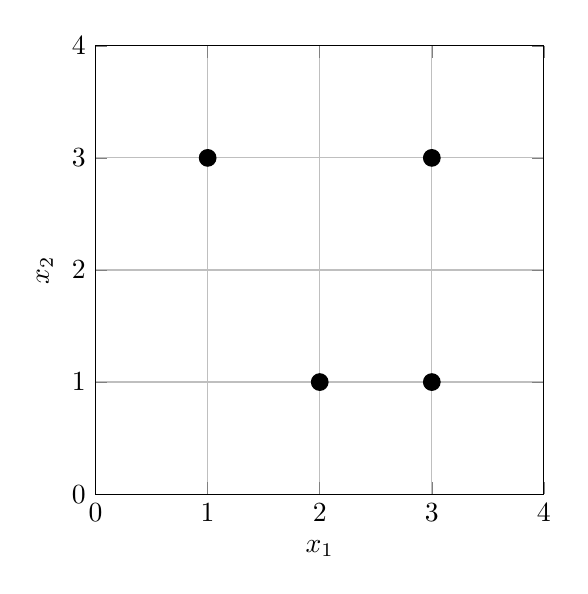
\begin{tikzpicture}
    \begin{axis}[
        scale=1, axis equal image, mark options={scale=1.5},
        xmin=0, xmax=4, xtick={0,...,4},
        ymin=0, ymax=4, ytick={0,...,4},
        grid=major, xlabel=$x_1$, ylabel=$x_2$]
        \addplot[scatter,
            only marks,
            point meta=explicit symbolic,
            scatter/classes={
                a={mark=*,black}
            }
        ] table [meta=label] {
            x y label
            1 3 a
            2 1 a
            3 1 a
            3 3 a
        };
    \end{axis}
    \end{tikzpicture} 
\end{center}
{%
    \checkboxchar{$\Box$} \checkedchar{$\blacksquare$} % change checkbox style locally
    \begin{checkboxes}
        \choice All linear decision boundaries
        \choice All axis-aligned rectangles i.e., rectangles where each side is parallel to either the x-axis or the y-axis
        \choice All \emph{squares} (note: these do not have to be axis-aligned)
        \choice All decision trees over $x_1$ and $x_2$
        \choice None of the above
    \end{checkboxes}
}
\begin{soln}
    C, D
\end{soln}
\begin{qauthor}
    Henry, heavily inspired by UNKNOWN
\end{qauthor} 


\part[2] \textbf{Select One:} What is the VC-dimension of a 1-nearest neighbor classifier on $D$-dimensional inputs? Assume the distance metric is Euclidean distance. Briefly justify your answer in 2-3 concise sentences. 
\begin{checkboxes}
    \choice $1$
    \choice $2$
    \choice $D$
    \choice $D+1$
    \choice $\infty$
\end{checkboxes}
\fillwithlines{6em}
\begin{soln}
    E; for any set of $N$ data points, a 1-NN can generate all possible labelings. To see this, fix an arbitrary labeling, use the original set of $N$ points as the training dataset and set the labels to be the desired labeling. 
\end{soln}
\begin{qauthor}
    Henry, heavily inspired by UNKNOWN
\end{qauthor} 

\begin{comment}
\begin{subparts}
    \subpart[]\textbf{Short answer:} Given a rectangular classifer (defined by four corner points), where all points inside the rectange are "+" and all points outside are "-", is it possible to shatter this dataset? Why or why not?
    \fillwithlines{6em}
    \begin{soln}
        Yes, we can rotate the rectangle (so it sits diagonally) to correctly classify $(1, 3), (3,1)$ as both being positive and the rest negative. Also, $(2,1), (3, 3)$ as both being positive and the rest negative.
    \end{soln}
    
    \subpart[]\textbf{Select one:} Using the same dataset above, what is the VC-dimension of a KNN classifier where $k=1$?
    \begin{checkboxes}
     \choice $1$ 
     \choice $2$
     \choice $3$
     \choice None of the above
    \end{checkboxes}
    \begin{soln}
        None of the above (Infinity)
    \end{soln}
\end{subparts}

\part[2] \textbf{Select all that apply:} Consider a finite-sized set $\Sc$ consisting of all unique binary feature vectors of length $M$. Let $\Hc_d$ be the hypothesis class of decision trees of maximum depth $d$, where each split is binary on the 0/1 values of a single feature. In which of the following cases could $\Hc_d$ shatter $\Sc$?
    {%
    \checkboxchar{$\Box$} \checkedchar{$\blacksquare$} % change checkbox style locally
    \begin{checkboxes}
     \choice $M$ = 1, $d$ = 1 \hspace{6em} (Reminder: depth $d$ is the length of the
     \choice $M$ = 2, $d$ = 2 \hspace{6em} longest path from the root to a leaf.)
     \choice $M$ = 2, $d$ = 3
     \choice $M$ = 3, $d$ = 2
     \choice None of the above 
    \end{checkboxes}
    }
    \begin{soln}
        A, B, C
    \end{soln}
    \begin{qauthor}
        Tanvi, Check if students understood the concept of shattering a classifier. I also have an idea to complicate this further by bringing in VC dimension if it's too easy.
    \end{qauthor}
    \begin{qtester}
     Good question! there is a lot to understand in order to figure this out!
    \end{qtester}


\part[2] \textbf{Select all that apply:} Recall the PAC learning bound for the finite, realizable case:
%
\textit{
For a finite hypothesis set $\mathcal{H}$ s.t. $c^* \in \mathcal{H}$, if the number of training data points satisfies 
$N \geq \frac{1}{\epsilon} \bigg( \ln(|\mathcal{H}|) + \ln\Big(\frac{1}{\delta}\Big) \bigg)$
then with probability at least $1-\delta$, all $h \in \mathcal{H}$ with $\hat{R}(h) = 0$ have $R(h) \leq \epsilon$.
}

If instead, $N = \frac{1}{2} \cdot \frac{1}{\epsilon} ( \ln(|\mathcal{H}|) + \ln (\frac{1}{\delta}) )$, which of the following hold with probability at least $1 - \delta$?
{%
    \checkboxchar{$\Box$} \checkedchar{$\blacksquare$} % change checkbox style locally
    \begin{checkboxes}
     \choice No $h \in \mathcal{H}$ with zero training error can have $R(h) \leq \epsilon$.
     \choice At least one $h \in \mathcal{H}$ with zero training error has $R(h) \leq \epsilon$.
     \choice All $h \in \mathcal{H}$ with zero training error have $R(h) \leq 2\epsilon$.
     \choice At least one $h \in \mathcal{H}$ with zero training error has $R(h) > \epsilon$.
     \choice None of the above
    \end{checkboxes}
}
\begin{soln}
    C
\end{soln}
\begin{qauthor}
    Alex, Define PAC and explain what it means to be approximately correct and what occurs with high probability
\end{qauthor}


\part[1] \textbf{Short answer:} In practice, training error $\widehat{R}(h)$ tends to decrease as we increase model complexity (e.g., VC-dimension). Describe in detail how the true error $R(h)$ is related to model complexity.
    \fillwithlines{6em}
    \begin{soln}
        True error tends to decrease with model complexity to a point, after which it starts increasing.
    \end{soln}
    \begin{qauthor}
    Emaan, Learning Objective: Theoretically justify regularization. Lecture 16, slide 29 (Learning Theory and Model Selection).
    \end{qauthor}
        
\part[1] \textbf{Short answer:} During training, describe one technique we can use to limit model complexity while still achieving good true error in the end. For full credit, clearly identify how this technique limits model complexity as represented by VC Dimension. 
    \fillwithlines{6em}
    \begin{soln}
        We should use a regularizer to tradeoff between complexity and error. Regularization reduces the VC dimension, allowing us to find the best tradeoff point.
    \end{soln}
    \begin{qauthor}
    Emaan, Learning Objective: Theoretically justify regularization. Lecture 16, slide 29 (Learning Theory and Model Selection).
    \end{qauthor}    
\end{comment}

\end{parts}
\clearpage
\sectionquestion{Societal Impacts of ML}

\begin{parts}

% Question 9
\part[1] \textbf{Select one:} Suppose we have a model that has a 0.5 error rate on each of two distinct groups in the dataset. Which of the following fairness metrics will \textbf{always} be satisfied? 

    % \checkboxchar{$\Box$} \checkedchar{$\blacksquare$}
    \begin{checkboxes}
        \choice False Negative Rate (FNR) parity
        \choice False Positive Rate (FPR) parity
        % \choice Negative Predictive Value (NPV) parity
        % \choice Positive Predictive Value (PPV) parity
        \choice Error parity 
        % \choice Statistical parity (or Selection rate parity)
        \choice A, B, and C
        \choice All of the above
        \choice None of the above
    \end{checkboxes}

    \begin{soln}
        (c) Error parity
    \end{soln}
    \begin{qauthor}
        Annie, fairness metrics and societal impacts
    \end{qauthor}

% Question 10
\part Markov is trying to build a model on predicting whether Cognitive Machine University (CMU') will admit a student. They are given the following dataset, split into two groups (Red/Blue), with entirely binary features.
    \begin{itemize}
        \item \textbf{GPA above 3.7:} 1 indicates that the student has a GPA above 3.7 reported on their application, 0 otherwise
        \item \textbf{Legacy:} takes on the value 1 if the student comes from a legacy family, 0 otherwise
        \item \textbf{Athelete:} 1 if student is recruited for sports, 0 otherwise
        \item \textbf{Admitted?:} shows the true label, 1 meaning the student was actually admitted, 0 otherwise
    \end{itemize}

    \begin{table}[htbp]
    \centering
    % \caption{Data Table}
    \label{tab:data}
    \begin{tabular}{|c|c|c|c|c|}
        \toprule
        Protected Attribute & GPA above 3.7 & Legacy & Athelete & Admitted? \\
        \midrule
        Red & 1 & 0 & 1 & 1 \\
        Red & 0 & 1 & 0 & 0 \\
        Red & 1 & 0 & 0 & 0 \\
        Red & 0 & 1 & 1 & 0 \\
        Red & 1 & 0 & 0 & 1 \\
        \midrule
        Blue & 0 & 0 & 1 & 0 \\
        Blue & 1 & 1 & 0 & 1 \\
        Blue & 0 & 0 & 0 & 1 \\
        Blue & 1 & 0 & 1 & 0 \\
        Blue & 0 & 1 & 0 & 0 \\
        \bottomrule
    \end{tabular}
\end{table}

Markov uses a model where we predict 1 if the ``majority" of the features for a student is 1 (i.e. at least 2 of the features has value 1 for that student), and 0 otherwise.

\clearpage
\begin{subparts}
    \subpart[1] \textbf{Numerical answer:} What is the negative predictive value on the Red group?

    \begin{tcolorbox}[fit,height=1cm, width=2cm, blank, borderline={1pt}{-2pt}]
    %solution
    \end{tcolorbox}
    \begin{soln}
    2/3
    \end{soln}

    \subpart[1] \textbf{Numerical answer:} What is the negative predictive value on the Blue group?
    \begin{tcolorbox}[fit,height=1cm, width=2cm, blank, borderline={1pt}{-2pt}]
    %solution
    \end{tcolorbox}
    \begin{soln}
    2/3
    \end{soln}

    \subpart[1] \textbf{True or False:} Does Markov's majority vote classifier achieve negative predictive value (NPV) parity?
    \begin{checkboxes}
     \choice True 
     \choice False
    \end{checkboxes}

    \begin{soln}
        True
    \end{soln}

    \subpart[1] \textbf{Numerical answer:} What is the false positive rate on the Red group?

    \begin{tcolorbox}[fit,height=1cm, width=2cm, blank, borderline={1pt}{-2pt}]
    %solution
    \end{tcolorbox}
    \begin{soln}
    1/3
    \end{soln}

    \subpart[1] \textbf{Numerical answer:} What is the false positive rate on the Blue group?
    \begin{tcolorbox}[fit,height=1cm, width=2cm, blank, borderline={1pt}{-2pt}]
    %solution
    \end{tcolorbox}
    \begin{soln}
    1/3
    \end{soln}

    \subpart[1] \textbf{True or False:} Does Markov's majority vote classifier achieve false positive rate (FPR) parity?
    \begin{checkboxes}
     \choice True 
     \choice False
    \end{checkboxes}

    \begin{soln}
        True
    \end{soln}

    \subpart[2] \textbf{Short answer:} Incorporating your responses from the previous parts, briefly discuss the fairness of the model. Can we say that the model is a fair between the Red and Blue groups?
    \fillwithlines{12em}
    \begin{soln}
    TODO: update this solution now that we compute NPV.
    
        Even though we achieve both false negative and false positive parity, it does not imply that this model is necessarily fair. There are other metrics we should test against (i.e. error parity, selection rate parity, etc.)
    \end{soln}

\clearpage
    \subpart[1] \textbf{Short answer:} What are some societal impacts of this model. In particular, what consequences might false negatives and false positive predictions have on the applicants?
    \fillwithlines{12em}
    \begin{soln}
    TODO: update this solution now that we compute NPV.
    
        A false negative mistake will take away a qualified student's acceptance to CMU, and a false positive mistake will admit non-qualified candidates to the university.
    \end{soln}
    
\end{subparts}

\begin{qauthor}
    Annie, societal impacts
\end{qauthor}



\end{parts}
\clearpage
%\sectionquestion{Miscellaneous}

\begin{parts}

\part[1] \textbf{Short answer:} Describe \textbf{one} topic \textbf{in detail} from the course material \textbf{in Lectures 17 - 25} that was \textbf{not covered on the exam}. For example, a learning objective that you reviewed that was not asked about here, a comparison of two algorithms or ML methods, etc. Write your answer in \textbf{3-5 sentences}.
\fillwithlines{18em}
\begin{soln}
    Accept pretty much anything that satisfies the above conditions.
\end{soln}
\begin{qauthor}
    Matt
\end{qauthor}
    
\end{parts}
    

% \clearpage
\end{questions}

\clearpage
\begin{center}
Do not remove this page! Use this page for scratch work.
\end{center}
\clearpage
\begin{center}
Do not remove this page! Use this page for scratch work.
\end{center}
\clearpage
\begin{center}
Do not remove this page! Use this page for scratch work.
\end{center}
\clearpage
\begin{center}
Do not remove this page! Use this page for scratch work.
\end{center}

\end{document}
